\documentclass[a4paper,10pt,dvipdfmx]{jsarticle}

\usepackage[dvipdfmx]{graphicx}
\usepackage{subcaption}
\usepackage{url}
\usepackage{bm}
\usepackage{amsmath,amssymb}
\usepackage{ascmac}

%\captionsetup[subfigure]{labelformat=simple}
\renewcommand{\thesubfigure}{(\alph{subfigure})}

\newcommand{\qed}{\hfill$\Box$}
\newcommand{\Proof}{\noindent{\bf Proof.}\quad}
\makeatletter
\newcommand{\figcaption}[1]{\def\@captype{figure}\caption{#1}}
\newcommand{\tblcaption}[1]{\def\@captype{table}\caption{#1}}
\makeatother

\newcommand{\bhline}[1]{\noalign{\hrule height #1}}  
\newcommand{\bvline}[1]{\vrule width #1}  

\begin{document}

\title{\vspace{-2cm}$\S$1.11 回帰係数の推定と検定}
\author{富島諒}
\date{2021年6月17日}

\maketitle

\section{回帰係数の推定と検定}

単回帰分析では説明変数の個数は1個であったが, 今回の節では説明変数が$p$個になり式\eqref{eq:model}のような回帰モデルとなると仮定する. ここで, $e_i$は独立な確率変数で正規分布$N(0, \sigma^2)$に従う. 
\begin{align}
  \label{eq:model}
  y_i = a_0 + a_1x_{1i} + \cdots + a_px_{pi}+e_i, \quad i=1, 2, \cdots
\end{align}

また, 標本のデータ$(x_{1i}, x_{2i}, \cdots, x_{pi}, y_i), i=1, 2, \cdots, n$であるとき, それに基づく回帰係数$\hat{a}_j$は$\S1.5$線形重回帰より, 式\eqref{eq:regre1}のように表される.
\begin{eqnarray}
  \label{eq:regre1}
  \hat{a}_j &= &
  \cfrac{
    \left|
      \begin{array}{cccccc}
      s_{11} &s_{12} &\cdots &s_{y1} &\cdots &s_{1p} \\
      s_{21} &s_{22} &\cdots &s_{y2} &\cdots &s_{2p} \\
      \vdots &\vdots &\ddots &\vdots &\ddots &\vdots \\
      s_{p1} &s_{p2} &\cdots &s_{yp} &\cdots &s_{pp}
      \end{array}
    \right|
  }
  {
    \left|
      \begin{array}{cccccc}
      s_{11} &s_{12} &\cdots &s_{1j} &\cdots &s_{1p} \\
      s_{21} &s_{22} &\cdots &s_{2j} &\cdots &s_{2p} \\
      \vdots &\vdots &\ddots &\vdots &\ddots &\vdots \\
      s_{p1} &s_{p2} &\cdots &s_{pj} &\cdots &s_{pp}
      \end{array}
    \right|
  }\\
  \notag 
  \\
  \notag
  & \quad &\text{($\ast \; j$列を$y$と$x_1, \cdots, x_p$との共分散に置き換えている)}
\end{eqnarray}

\begin{itembox}[l]{余因子と余因子展開}
   \quad $p\geq 2$とする. $p$次正方行列$\bm{V}=[s_{jl}]$の第$j$行と第$l$列を取り除いてできる$p-1$次正方行列の行列式を$(-1)^{j+l}$倍した数, 
   \begin{align*}
    \left|
      \begin{array}{cccccc}
        s_{11} &\cdots &s_{1(l-1)} &s_{1(l+1)} &\cdots &s_{1p} \\
        \vdots &\ddots &\vdots &\ddots &\vdots &\cdots \\
        s_{(j-1)1} &\cdots &s_{(j-1)(l-1)} &s_{(j-1)(l+1)} &\cdots &s_{(j-1)p} \\
        s_{(j+1)1} &\cdots &s_{(j+1)(l-1)} &s_{(j+1)(l+1)} &\cdots &s_{(j+1)p} \\
        \vdots &\ddots &\vdots &\ddots &\vdots &\cdots \\
        s_{p1} &\cdots &s_{p(l-1)} &s_{p(l+1)} &\cdots &s_{pp} \\
      \end{array}
    \right|(-1)^{j+l}
  \end{align*}
  を$\bm{V}$の$(j, l)${\bf 余因子}といい, $V_{jl}$と表す.  

  \quad また行列$\bm{V}$に対して, 
  \begin{align}
    \label{eq:cofacE1}
    |\bm{V}| &= s_{j1}V_{j1} + s_{j2}V_{j2} + \cdots + s_{jp}V_{jp} 
    \text{\quad (第j行に関する展開)}\\
    \label{eq:cofacE2}
    |\bm{V}| &= s_{1l}V_{1l} + s_{2l}V_{2l} + \cdots + s_{pl}V_{pl} 
    \text{\quad (第l列に関する展開)}
  \end{align}
  のような変換を行える. これを{\bf 余因子展開}という.  
\end{itembox}

ここで式\eqref{eq:regre1}の分子で余因子展開の定理\eqref{eq:cofacE2}を用い, 分母は$\S1.5$で定義された分散共分散行列$\bm{V}$であるから, 式\eqref{eq:regre1}は式\eqref{eq:regre2}のように変形できる. 

\begin{eqnarray}
  \label{eq:regre2}
  \hat{a}_j =
  \cfrac{
    \left|
      \begin{array}{cccccc}
      s_{11} &s_{12} &\cdots &s_{y1} &\cdots &s_{1p} \\
      s_{21} &s_{22} &\cdots &s_{y2} &\cdots &s_{2p} \\
      \vdots &\vdots &\ddots &\vdots &\ddots &\vdots \\
      s_{p1} &s_{p2} &\cdots &s_{yp} &\cdots &s_{pp}
      \end{array}
    \right|
  }
  {
    \left|
      \begin{array}{cccccc}
        s_{11} &s_{12} &\cdots &s_{1j} &\cdots &s_{1p} \\
        s_{21} &s_{22} &\cdots &s_{2j} &\cdots &s_{2p} \\
        \vdots &\vdots &\ddots &\vdots &\ddots &\vdots \\
        s_{p1} &s_{p2} &\cdots &s_{pj} &\cdots &s_{pp}
        \end{array}
    \right|
  }
  = \frac{s_{y1}V_{1j}+s_{y2}V_{2j}+\cdots +s_{yp}V_{pj}}{|\bm{V}|}
\end{eqnarray}

\begin{itembox}[l]{余因子行列と逆転公式}
  \ $p$次正方行列$\bm{V}=[s_{jl}]$とする. $\bm{V}$の{\bf 余因子行列}$\tilde{\bm{V}}$とは, $(j, l)$成分に余因子$V_{jl}$を持つ$p$次正方行列の転地行列である. したがって, $\tilde{\bm{V}}$は式\eqref{eq:adj_mat}のようになる. 
  \begin{align}
    \label{eq:adj_mat}
    \tilde{\bm{V}} =
    \left[
      \begin{array}{cccc}
        V_{11} &V_{12} &\cdots &V_{1p} \\
        V_{21} &V_{22} &\cdots &V_{2p}\\
        \vdots &\vdots &\ddots &\vdots\\
        V_{p1} &V_{p2} &\cdots &V_{pp} \\
      \end{array}
    \right]^\top
    = 
    \left[
      \begin{array}{cccc}
        V_{11} &V_{21} &\cdots &V_{p1} \\
        V_{12} &V_{22} &\cdots &V_{p2}\\
        \vdots &\vdots &\ddots &\vdots\\
        V_{1p} &V_{2p} &\cdots &V_{pp} \\
      \end{array}
    \right]
  \end{align}

そして, 正方行列$\bm{V}$に対して式\eqref{eq:inv}のような関係式が成り立つ. これを{\bf 逆転公式}という. 
  \begin{align}
    \label{eq:inv}
    \bm{V}^{-1} = \frac{\tilde{\bm{{V}}}}{|\bm{V}|}
  \end{align}
\end{itembox}
そして, $\bm{V}$の逆行列の$(j, l)$要素を$s^{jl}$とすると, 逆転公式の式\eqref{eq:inv}より, 
\begin{align*}
  \bm{V}^{-1}
  &=  \frac{\tilde{\bm{{V}}}}{|\bm{V}|}\\
  \left[
    \begin{array}{cccc}
      s^{11} &s^{12} &\cdots &s^{1p}\\
      s^{21} &s^{22} &\cdots &s^{2p} \\
      \vdots &\vdots &\ddots &\vdots \\
      s^{p1} &s^{p2} &\cdots &s^{pp}\\
    \end{array}
  \right]
  &=
  \left[
    \begin{array}{cccc}
      V_{11} &V_{21} &\cdots &V_{p1} \\
      V_{12} &V_{22} &\cdots &V_{p2}\\
      \vdots &\vdots &\ddots &\vdots\\
      V_{1p} &V_{2p} &\cdots &V_{pp} \\
    \end{array}
  \right]
  / |\bm{V}|
\end{align*}
となるので, $s^{jl}=\frac{V_{lj}}{|\bm{V}|}$である. したがって, 式\eqref{eq:regre2}は, 

\begin{align}
  \tag{\ref{eq:regre2}}
  \hat{a}_{j} %回帰係数\hat{a}_jの変形
  &= \frac{s_{y1}V_{1j}+s_{y2}V_{2j}+\cdots +s_{yp}V_{pj}}{|\bm{V}|} \\
  \notag 
  &= s_{y1}s^{j1}+s_{y2}s^{j2}+\cdots +s_{yp}s^{jp} \\
  \notag 
  &= \sum_{l=1}^ps_{yl}s^{jl} \\
  \notag 
  &= \sum_{l=1}^ps^{jl}\frac{1}{n}\sum_{i=1}^n(y_i-\bar{y})(x_{li}-\bar{x}_l) \\
  \notag 
  &= \sum_{l=1}^ps^{jl}\frac{1}{n}\left\{
      \sum_{i=1}^n(x_{li}-\bar{x}_l)y_i
      - \bar{y}\sum_{i=1}^n(x_{li}-\bar{x}_l)
    \right\} \\
  \label{eq:j_regressionC}
   &= \frac{1}{n}\sum_{l=1}^p\sum_{i=1}^ns^{jl}(x_{li}-\bar{x}_l)y_i
\end{align}
となる. また, $\S1.5$で
\begin{align}
  \label{eq:sec5_y_bar} %目的変数\bar{y}の平均の変形
  \hat{a}_0 = \bar{y}-(\hat{a}_1\bar{x}_1+\cdots+\hat{a}_p\bar{x}_p)
\end{align}
のような式が得られたので, これに式\eqref{eq:j_regressionC}を代入すると, 
\begin{align}
  \notag \hat{a}_0 %定数項の回帰係数\hat{a}_0
  &= \bar{y}-(\hat{a}_1\bar{x}_1+\cdots+\hat{a}_p\bar{x}_p) \\
  \notag 
  &= \bar{y}-\sum_{j=1}^p\hat{a}_j\bar{x}_j \\
  \notag 
  &= \frac{1}{n}\sum_{i=1}^ny_i-\frac{1}{n}\sum_{j=1}^p\sum_{i=1}^n\sum_{l=1}^p\bar{x}_js^{jl}(x_{li}-\bar{x}_l)y_i \\
  \label{eq:0_regressionC}
  &=\frac{1}{n}\sum_{i=1}^n\left\{
      1-\sum_{j=1}^p\sum_{l=1}^p\bar{x}_js^{jl}(x_{li}-\bar{x}_l)
    \right\}y_i
\end{align}
のようになる. 

したがって, $\hat{a}_j, \hat{a}_0$正規分布に従う変数$y_i, i=1, 2, \cdots, n$の1次式で表されることがわかる. これより回帰係数$\hat{a}_j$及び定数項$\hat{a}_0$の期待値と分散を求めると, 式\eqref{eq:regre_3}のようになる. 

\begin{subequations}
  \label{eq:regre_3}
  \begin{alignat}{2}
    \label{eq:e_j} %回帰係数\hat{a}_jの期待値
    &\operatorname{E}(\hat{a}_j) = a_j, &  &j=1, 2, \cdots, p \\
    \label{eq:v_j} %回帰係数\hat{a}_jの分散
    &\operatorname{V}(\hat{a}_j) = \frac{s^{jj}\sigma^2}{n},& &j=1, 2, \cdots, p \\
    \label{eq:cov_jl} %回帰係数\hat{a}_jと\hat{a}_lの共分散
    &\operatorname{Cov}(\hat{a}_j, \hat{a}_l) =\frac{s^{jl}\sigma^2}{n},& &j\neq l,\; j, l=1, 2, \cdots, p\\
    \label{eq:e_0} %定数項の回帰係数\hat{a}_0の期待値
    &\operatorname{E}(\hat{a}_0)=a_0 \\
    \label{eq:v_0} %定数項の回帰係数\hat{a}_0の分散
    &\operatorname{V}(\hat{a}_0) = \left(\frac{1}{n}+\sum_{j=1}^p\sum_{l=1}^p\frac{\bar{x}_j\bar{x}_ls^{jl}}{n}\right)\sigma^2 \\
    \label{eq:cov_0j} %定数項の回帰係数\hat{a}_0と\hat{a}_jの共分散
    &\operatorname{Cov}(\hat{a}_0, \hat{a}_j) = -\sum_{l=1}^p\frac{\bar{x}_ls^{jl}\sigma^2}{n},&\quad & j=1, 2, \cdots, p 
  \end{alignat}
\end{subequations}

なお, 式\eqref{eq:regre_3}の証明は長くなるので後述する(\ref{sec:6siki}). 式\eqref{eq:e_j}と式\eqref{eq:e_0}より標本のデータを用いて計算した$\hat{a}_0, \hat{a}_1, \cdots, \hat{a}_p$は母集団における値$a_0, a_1, \cdots, a_p$に対して不偏推定値となっていることが言える. 

\begin{itembox}[l]{不偏推定値}
  \quad 標本から測定した推定値の期待値が母集団のそれに等しいとき、その推定値を{\bf 不偏推定値(量)}という.  
\end{itembox} \\

単回帰の場合と同様, 
\begin{align}
  \label{eq:norm_s}
  u = \frac{\hat{a}_j-\operatorname{E}(\hat{a}_j)}{\sqrt{\operatorname{V}(\hat{a}_j)}}
\end{align}
のように標準化すると$u$は標準正規分布$N(0, 1)$に従う. またこの時, 分母に含まれる未知の誤差分散$\sigma^2$を不偏推定値
\begin{align}
  \label{eq:unbiasedV} %誤差分散
  \operatorname{V}_e = \frac{\operatorname{F}(\hat{a}_0, \hat{a}_1, \cdots, \hat{a}_p)}{n-p-1}
\end{align}
で置き換えて得られる統計量, 
\begin{align}
  \label{eq:stat_j}
  t &= \frac{\hat{a}_j-a_j}{\sqrt{s^{jj}\frac{\operatorname{V}_e}{n}}} \\
  \label{eq:stat_0}
  t &= \frac{\hat{a}_0-a_0}{\sqrt{\left(1+\sum_{j=1}^p\sum_{l=1}^p\bar{x}_j\bar{x}_ls^{jl}\right)\frac{\operatorname{V}_e}{n}}}
\end{align}
はいずれも自由度$n-p-1$のt分布に従う. また, 式\eqref{eq:unbiasedV}の$\operatorname{V}_e$が誤差分散$\sigma^2$の不偏推定値であることの証明は後述する(\ref{sec:ve_unbiased}).

ここで式\eqref{eq:unbiasedV}における右辺の分子である予測誤差の平方和は
\begin{align}
  \notag
  \operatorname{F}(\hat{a}_0, \hat{a}_1, \cdots, \hat{a}_p) 
  &= \sum_{i=1}^p\left\{
    y_i-(\hat{a}_0+\hat{a}_1x_{1i}+\cdots+\hat{a}_px_{pi})
  \right\}^2 \text{\; ($\S1.5$より)}\\
  \label{eq:f_dist} 
  &= n(s_{yy}-\sum_{l=1}^ps_{yl}\hat{a}_l)
\end{align}
のように変形できる. 証明は後述する(\ref{sec:mean_squared_error_sum}).

これより, 仮説$\operatorname{H}_0:a_j=a_j^{(0)}$あるいは$\operatorname{H}_0:a_0=a_0^{(0)}$の検定($a_j^{(0)}, a_0^{(0)}$は与えられた値)及び$\hat{a}_j, \hat{a}_0$の信頼区間は次のようになる. 

\subsubsection*{$\bullet \; $仮説$\operatorname{H}_0:a_j=a_j^{(0)}$の検定$(j=1, 2, \cdots, p)$:}
  \begin{align}
    \label{eq:hypo_j}
    |t| = \frac{|\hat{a}_j-a_j^{(0)}|}{\sqrt{s^{jj}\frac{\operatorname{V}_e}{n}}} \geq t_{\alpha}(n-p-1) 
  \end{align} 
ならば危険率$\alpha$で仮説を棄却し, 不等号の向きが逆ならば仮説を採択.

\subsubsection*{$\bullet \; $仮説$\operatorname{H}_0:a_0=a_0^{(0)}$の検定:}
  \begin{align}
    \label{eq:hypo_0}
    |t| = \frac{|\hat{a}_0-a_0^{(0)}|}{\sqrt{\left(1+\sum_{j=1}^p\sum_{l=1}^p\bar{x}_j\bar{x}_ls^{jl}\right)\frac{\operatorname{V}_e}{n}}} \geq
    t_{\alpha}(n-p-1) 
  \end{align} 
ならば危険率$\alpha$で仮説を棄却し, 不等号の向きが逆ならば仮説を採択. 

\subsubsection*{$\bullet \; a_j, j=1, 2, \cdots, p$の信頼率$1-\alpha$の信頼区間:}
  \begin{align}
    \label{eq:CI_j}
    \hat{a}_j-t_{\alpha}(n-p-1)\sqrt{\frac{s^{jj}\operatorname{V}_e}{n}}\leq a_j 
    \leq \hat{a}_j+t_{\alpha}(n-p-1)\sqrt{\frac{s^{jj}\operatorname{V}_e}{n}}
  \end{align}

\subsubsection*{$\bullet \; a_0$の信頼率$1-\alpha$の信頼区間:}
  \begin{align}
    \label{eq:CI_0}
    \begin{split}
      \hat{a}_0-t_{\alpha}(n-p-1)\sqrt{\left(1+\sum_{j=1}^p\sum_{l=1}^p\bar{x}_j\bar{x}_ls^{jl}\right)\frac{\operatorname{V}_e}{n}} \leq a_0\\
      \leq \hat{a}_0+t_{\alpha}(n-p-1)\sqrt{\left(1+\sum_{j=1}^p\sum_{l=1}^p\bar{x}_j\bar{x}_ls^{jl}\right)\frac{\operatorname{V}_e}{n}}
    \end{split}
  \end{align}\\

\begin{itembox}[l]{信頼区間と仮説}
  \ 母集団から標本をとってきて, その平均から$100(1-\alpha)\%$という作業を求めるという作業を行ったとき$100(1-\alpha)$回, 母平均が含まれるような区間を{\bf 信頼区間}という.\\ 
  
  \ また, t分布による両側検定を行い, 検定統計量が自由度と標本の個数に基づく値より大きければ(外側にある)その仮説を棄却する. 逆に, 小さければ仮説を採択する.

  \ 例えば, 自由度が9のt分布において危険率$5\%$では$t_{0.025}(9)=2.26$となる.検定統計量によって求めた値が$t=3.00$であるとすると, 図\ref{fig:kasetsu}より, 有意水準$5\%$において帰無仮説を棄却することとなる.
\end{itembox}

\begin{figure}[htb]
  \centering
  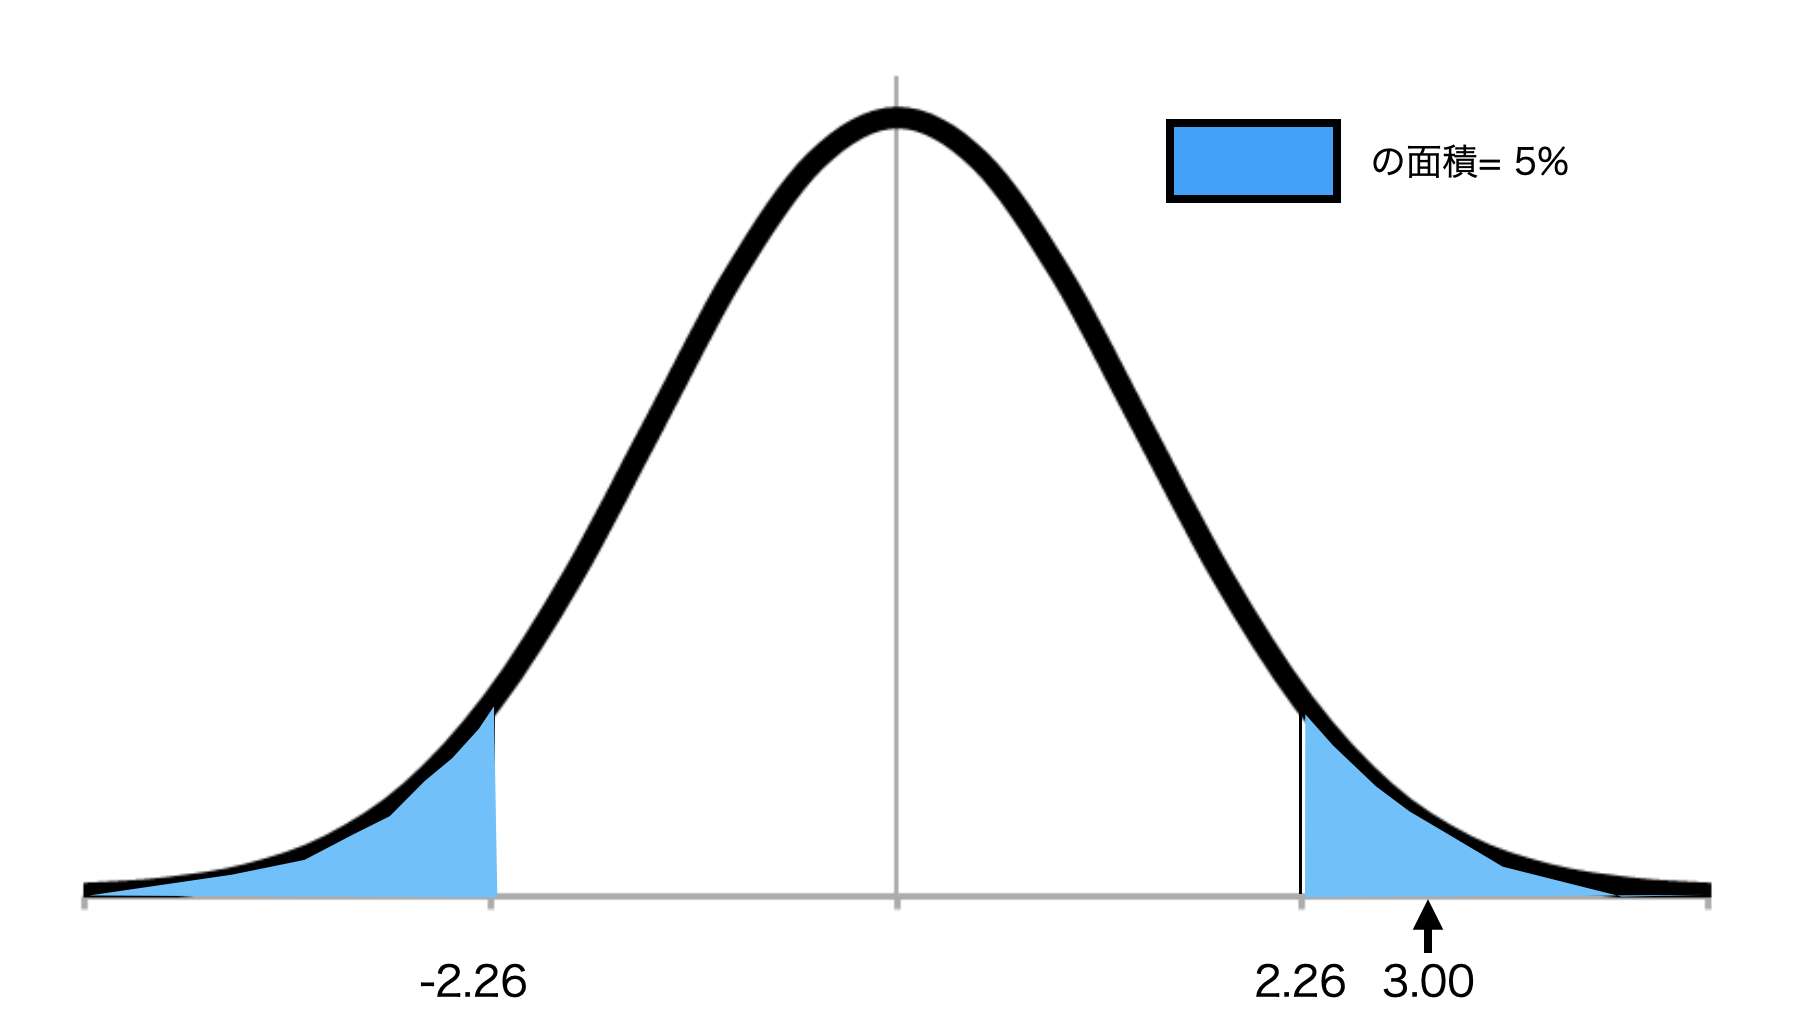
\includegraphics[width=10cm]{../pics/kasetsu.png}
  \caption{t分布による仮説検定}
  \label{fig:kasetsu}
\end{figure}

\newpage

次に, 回帰の有意性, 言い換えると, 取り上げた説明変数$x_1, \cdots, x_p$が全体として$y$の予測に役立つと言えるのかどうかの検定問題を考える. まず, 予測値$Y_i$は指定変数の組$(x_{1i}, x_{2i}, \cdots, x_{pi})$に対して
\begin{align}
  \label{eq:prediction}
  Y_i = \hat{a}_0 + \hat{a}_1x_{1i} + \cdots + \hat{a}_px_{pi}
\end{align}
のように計算される. そして, 観測値$y_i$の変動(平方和)を式\eqref{eq:sum_of_square}のように分解する.
\begin{align}
  \notag
  \sum_{i=1}^n(y_i-\bar{y})^2 
  &= \sum_{i=1}^n(y_i-\bar{Y})^2 \\
  \notag
  &\text{\quad ($\because$ 
  \; $\bar{y}= \frac{1}{n}\sum_{i=1}^ny_i = \frac{1}{n}\sum_{i=1}^nY_i + \frac{1}{n}\sum_{i=1}^ne_i = \frac{1}{n}\sum_{i=1}^nY_i = \bar{Y}$より)} \\
  \notag
  &= \sum_{i=1}^n(y_i-Y_i + Y_i-\bar{Y})^2 \\
  \label{eq:sum_of_square}
  &= \sum_{i=1}^n(y_i-Y_i)^2+\sum_{i=1}^n(Y_i-\bar{Y})^2 +2\sum_{i=1}^n(y_i-Y_i)(Y_i-\bar{Y})
\end{align}
また, $\S1.5$で次のような関係となることがわかっている. 
\begin{align}
  \label{eq:ch5_19}
    \begin{cases}
      \displaystyle
      \sum_{i=1}^n  \left\{
      (y_i-\bar{y})-\hat{a}_1(x_{1i}-\bar{x}_1)-\hat{a}_2(x_{2i}-\bar{x}_2)-\cdots -\hat{a}_p(x_{pi}-\bar{x}_p)
    \right\} = 0 \\
    \displaystyle
    \sum_{i=1}^n  \left\{
      (y_i-\bar{y})-\hat{a}_1(x_{1i}-\bar{x}_1)-\hat{a}_2(x_{2i}-\bar{x}_2)-\cdots -\hat{a}_p(x_{pi}-\bar{x}_p)\right
    \}x_{1i} = 0 \\
    \qquad \vdots \\
    \displaystyle
    \sum_{i=1}^n  \left\{
      (y_i-\bar{y})-\hat{a}_1(x_{1i}-\bar{x}_1)-\hat{a}_2(x_{2i}-\bar{x}_2)-\cdots -\hat{a}_p(x_{pi}-\bar{x}_p)\right
    \}x_{ji} = 0\\
    \qquad \vdots \\
    \displaystyle
    \sum_{i=1}^n  \left\{
      (y_i-\bar{y})-\hat{a}_1(x_{1i}-\bar{x}_1)-\hat{a}_2(x_{2i}-\bar{x}_2)-\cdots -\hat{a}_p(x_{pi}-\bar{x}_p)\right
    \}x_{pi} = 0
    \end{cases}
\end{align}

式\eqref{eq:ch5_19}を用いると, 式\eqref{eq:sum_of_square}の第3項は
\begin{align}
  \notag
    \sum_{i=1}^n(y_i-Y_i)(Y_i-\bar{Y}) 
    &= \sum_{i=1}^n\left\{
      y_i-(\hat{a}_0+\hat{a}_1x_{1i}+\cdots +\hat{a}_px_{pi})
    \right\}
    \left\{
      \hat{a}_0 +\hat{a}_1x_{1i}+\cdots \hat{a}_px_{pi}-\bar{Y}
    \right\} \\
    \notag
    &=\sum_{i=1}^n\left\{
      (y_i-\bar{y})-\hat{a}_1(x_{1i}-\bar{x}_1)-\cdots -\hat{a}_p(x_{pi}-\bar{x}_p)
    \right\}
    \left\{
      \hat{a}_0+\hat{a}_1x_{1i}+\cdots \hat{a}_px_{pi}-\bar{Y}
    \right\} \\
    \notag
    & \text{\quad ($\because$ 式\eqref{eq:sec5_y_bar}
    \; $\hat{a}_0 = \bar{y}-(\hat{a}_1\bar{x}_1+\cdots+\hat{a}_p\bar{x}_p)$より)} \\
    &= 0 
\end{align}
したがって, 式\eqref{eq:sum_of_square3}のように変動の分解ができる. 
\begin{align}
  \label{eq:sum_of_square3}
  \underbrace{\sum_{i=1}^n(y_i-\bar{y})^2}_{全変動(S_T)} = &\underbrace{\sum_{i=1}^n(Y_i-\bar{Y})^2}_{回帰変動(S_R)}+\underbrace{\sum_{i=1}^n(y_i-Y_i)^2}_{残差変動(S_e)}
\end{align}

右辺の第1項$\operatorname{S}_R$は回帰式に基づく予測値$Y_i$の変動, 第2項$\operatorname{S}_e$は残差の変動であって, 前者は全変動のうち回帰によって説明される部分, 後者は説明されない部分の変動である. もし取り上げた説明変数$x_1, \cdots, x_p$が$y$の予測に有効であるとすれば, 全変動$S_T$は一定であるため残差変動$S_e$は小さくなり, 逆に無効であるとすれば, $S_e$は大きくなる. ここで
\begin{align}
  \label{eq:coefficient_of_determination}
  \operatorname{R}^2 = \frac{\operatorname{S}_R}{\operatorname{S}_T} = \frac{\sum_{i=1}^n(Y_i-\bar{Y})^2}{\sum_{i=1}^n(y_i-\bar{y})^2}
\end{align}
のようにおけば, $\operatorname{R}^2$は全体の変動のうち回帰によって説明される部分の大きさの割合を表し, その意味で{\bf 決定係数}あるいは{\bf 寄与率}と呼ばれる. また, $\operatorname{S}_e$は最小化された予測誤差の平方和$\operatorname{F}(\hat{a}_0, \hat{a}_1, \cdots , \hat{a}_p)$に等しい.

そして, $\S1.7$で重相関係数$r_{y・12\cdots p}$は
\begin{align*}
  r_{y・12\cdots p} = \frac{s_{yY}}{\sqrt{s_{yy}s_{YY}}}
\end{align*}
のように表せた. これを2乗した式\eqref{eq:mul_correlation_coefi}を考える. 
\begin{align}
  \label{eq:mul_correlation_coefi}
  r_{y・12\cdots p}^2 
  &= \frac{s_{yY}^2}{s_{yy}s_{YY}} 
\end{align}
ここで, 
\begin{align}
  \notag
  s_{yY} &= \frac{1}{n}\sum_{i=1}^n(y_i-\bar{y})(Y_i-\bar{Y}) \\
  \notag
  &= \frac{1}{n}\sum_{i=1}^n(y_i-Y_i+Y_i-\bar{Y})(Y_i-\bar{Y}) \\
  \notag
  &= \frac{1}{n}\sum_{i=1}^n(e_i+Y_i-\bar{Y})(Y_i-\bar{Y}) \\
  \label{eq:cov_yY}
  &= \frac{1}{n}\sum_{i=1}^ne_i(Y_i-\bar{Y})+\frac{1}{n}\sum_{i=1}^n(Y_i-\bar{Y})^2 
\end{align}

\begin{itembox}[l]{残差の性質}
  残差$e_i = y_i - (a_0 + a_1x_{1i} + \cdots + a_px_{pi})$には次の2つの性質がある. 
  \begin{itemize}
    \item 残差の総和は0
    \begin{align}
      \label{eq:sum_ei}
      \sum_{i=1}^ne_i = 0
    \end{align}
    \item 説明変数$x_i$と残差$e_i$との積和は0
    \begin{align}
      \label{eq:sum_eixi}
      \sum_{i=1}^nx_{ji}e_i = 0
    \end{align}
  \end{itemize}
\end{itembox}

式\eqref{eq:cov_yY}の右辺第1項に関して, 
\begin{align}
  \notag
  \sum_{i=1}^ne_i(Y_i-\bar{Y})
  &= \sum_{i=1}^ne_iY_i-\bar{Y}\sum_{i=1}^ne_i  \\
  \notag
  &= \sum_{i=1}^ne_i(\hat{a}_0+\hat{a}_1x_{1i}+\cdots + \hat{a}_px_{pi}) \text{\quad ($\because$ 式\eqref{eq:sum_ei} \;$\sum_{i=1}^ne_i = 0$より)}\\
  \notag
  &= \hat{a}_0\sum_{i=1}^ne_i+\hat{a}_1\sum_{i=1}^ne_ix_{1i}+\cdots +\hat{a}_p\sum_{i=1}^ne_ix_{pi} \\
  \label{eq:residual_err}
  &= 0 
  \text{\quad ($\because$ 式\eqref{eq:sum_eixi} \;$\sum_{i=1}^nx_{ji}e_i = 0$より)}
\end{align}
したがって, 式\eqref{eq:cov_yY}は式\eqref{eq:residual_err}の結果から, 
\begin{align}
  \tag{\ref{eq:cov_yY}}
  s_{yY} 
  &= \frac{1}{n}\sum_{i=1}^ne_i(Y_i-\bar{Y})+\frac{1}{n}\sum_{i=1}^n(Y_i-\bar{Y})^2 \\
  \label{eq:syY2sYY}
  &= \frac{1}{n}\sum_{i=1}^n(Y_i-\bar{Y})^2 = s_{YY}
\end{align}
式\eqref{eq:syY2sYY}の結果より, $s_{yY}=s_{YY}$であるから, 式\eqref{eq:mul_correlation_coefi}は
\begin{align}
  \tag{\ref{eq:mul_correlation_coefi}}
  r_{y・12\cdots p}^2 
  &= \frac{s_{yY}^2}{s_{yy}s_{YY}} \\
  \notag 
  &= \frac{s_{YY}^2}{s_{yy}s_{YY}} \\
  \notag 
  &= \frac{s_{YY}}{s_{yy}} \\
  \notag 
  &= \frac{\sum_{i=1}^n(Y_i-\bar{Y})^2}{\sum_{i=1}^n(y_i-\bar{y})^2} \\
  \label{eq:r2_R2}
  &= \operatorname{R^2}
\end{align}
となり, 重相関係数$r_{y・12\cdots p}$の2乗は決定係数$\operatorname{R}^2$と等しくなる.  \\

\begin{itembox}[l]{$\chi^2$分布}
  $Z_1, Z_2, \cdots, Z_k$が互いに独立で標準正規分布$N(0, 1)$に従う確率変数であるとき, 次の式は{\bf $\chi^2$分布}に従うという. 
  \begin{align*}
    \chi^2 = Z_1^2 + Z_2^2 + \cdots + Z_k^2
  \end{align*}
\end{itembox}

モデルが適合しているとき$\sum(y_i-Y_i)^2/\sigma^2$は, 
\begin{align*}
  \sum(y_i-Y_i)^2/\sigma^2 = \sum(e_i-0)^2/\sigma^2
\end{align*}
となるので自由度$n-p-1$のカイ2乗分布に従う. また特に説明変数$x_1, \cdots, x_p$が$y$の予測に何ら寄与しない, 言い換えれば母集団における回帰係数の値が$a_1=\cdots = a_p=0$のときには, 
回帰の変動は
\begin{align*}
  \sum_{i=1}^{n}(Y_i-\bar{Y})^2
  &= \sum_{i=1}^{n}\left\{
    (\hat{a}_0 + \hat{a}_{1}x_{1i} + \cdots + \hat{a}_{p}x_{pi})
    - (\hat{a}_0 + \hat{a}_{1}\bar{x}_1 + \cdots + \hat{a}_{p}\bar{x}_p)
  \right\}^2 \\
  &= \sum_{i=1}^{n} \left\{
    \hat{a}_1(x_{1i}-\bar{x}_1) + \cdots + \hat{a}_p(x_{pi}-\bar{x}_p)
  \right\}^2 \\
  &= \sum_{i=1}^{n} \sum_{j=1}^p \hat{a}_j^2(x_{ji} - \bar{x}_{j})^2
  + \sum_{i=1}^n\sum_{j=1}^p\sum_{l=1}^p \hat{a}_j\hat{a}_l(x_{ji}-\bar{x}_{j})(x_{li}-\bar{x}_l) \qquad (j\neq l)\\
  &= n\sum_{j=1}^p \hat{a}_j^2s_{jj} 
  + n\sum_{j=1}^p\sum_{l=1}^p\hat{a}_j\hat{a}_ls_{jl} 
\end{align*}
$\operatorname{V}(\hat{a}_j)=\frac{\sigma^2}{ns_{jj}}$, かつ, 説明変数$x_j, x_l$は互いに独立であることを用いると, 
\begin{align*}
  \sum_{i=1}^{n}(Y_i-\bar{Y})^2
  &= \sum_{j=1}^p\frac{\hat{a}_j^2\sigma^2}{\operatorname{V}(\hat{a}_j)} \\
  \frac{1}{\sigma^2}\sum_{i=1}^{n}(Y_i-\bar{Y})^2 
  &= \sum_{j=1}^p\frac{\hat{a}_j^2}{\operatorname{V}(\hat{a}_j)} \\
  &= \sum_{j=1}^p\left( \frac{\hat{a}_j}{\sqrt{\operatorname{V}(\hat{a}_j)}} \right)^2
\end{align*}
$u = \frac{\hat{a}_j -a_j}{\sqrt{\operatorname{V}(\hat{a}_j)}}\sim \operatorname{N}(0, 1)$において, $a_j=0, j=1, \cdots, p$と仮定すると, 
\begin{align*}
  u= \frac{\hat{a}_j}{\sqrt{\operatorname{V}(\hat{a}_j)}} \sim \operatorname{N}(0, 1)
\end{align*}
なので, 
\begin{align*}
  \sum_{j=1}^p\left( \frac{\hat{a}_j}{\sqrt{\operatorname{V}(\hat{a}_j)}} \right)^2
\end{align*}
は自由度$p$の$\chi^2$分布に従う. すなわち,
\begin{align*}
  \sum_{i=1}^n\frac{(Y_i - \bar{Y})^2}{\sigma^2}
\end{align*}
は$\sum(y_i-Y_i)^2/\sigma^2$とは独立に自由度$p$の$\chi^2$分布に従う.これより次のような分散分析表(表\ref{tab:anovo_table})が構成される. 

\begin{table}[htb]
  \centering
  \caption{分散分析表}
  \label{tab:anovo_table}
  \begin{tabular}{ccccc}\bhline{1.5pt}
   変動要因 &平方和 &自由度 &不偏分散 &分散比  \\ \hline
   回帰による &$\displaystyle \operatorname{S}_R=\sum_{i=1}^n(Y_i-\bar{Y})^2$ &$p$ &$\displaystyle \operatorname{V}_R = \frac{\operatorname{S}_R}{p}$ &$\displaystyle \operatorname{F}_0=\frac{\operatorname{V}_R}{\operatorname{V}_e}$  \\
   回帰からの &$\displaystyle \operatorname{S}_e=\sum_{i=1}^n(y_i-Y_i)^2$ &$n-p-1$ &$\displaystyle \operatorname{V}_e=\frac{\operatorname{S}_e}{n-p-1}$ & \\
   全体 &$\displaystyle \operatorname{S}_T=\sum_{i=1}^n(y_i-\bar{y})^2$ &$n-1$ & & \\ \hline
  \end{tabular}
\end{table}

この分散分析表において分散比$\operatorname{F}_0$が$\operatorname{F}_0\geq \operatorname{F}^p_{n-p-1}(\alpha)$ならば仮説$H_0: a_1=\cdots =a_p=0$は危険率$\alpha$で棄却され, 回帰が変動の大きな要因となっている(回帰が有意である)ため, 取り上げた説明変数は全体として$y$の予測に役立つ, と結論づけられる. ここで, $\operatorname{F}^p_{n-p-1}(\alpha)$は自由度$(p, n-p-1)$のF分布の上側$100\alpha\%$点である. 

\begin{itembox}[l]{F分布}
  \quad
  2つの確率分布$U, V$が次の条件を満たすとする. 
  \begin{description}
    \item[(i)] $U$は自由度$k_1$のカイ2乗分布$\chi^2(k_1)$に従う
    \item[(ii)] $V$は自由度$k_2$のカイ2乗分布$\chi^2(k_2)$に従う
    \item[(iii)] $U, V$は独立である. 
  \end{description}
  ここで, $U$と$V$をそれぞれの自由度で割って調整したあとにとった比, すなわちフィッシャー分散比を
  \begin{align*}
    \operatorname{F} = \frac{U/k_1}{V/k_2}
  \end{align*}
  と定義すると, $\operatorname{F}$が従う確率分布を自由度$(k_1, k_2)$のF分布といい, $\operatorname{F}_n^{k_1}$または$\operatorname{F}(k_1, k_2)$と表す. \\

  \quad 例えば, 回帰の自由度が3で残差の自由度が11であり, 分散比$\operatorname{F}_0=8.21$の場合, $\operatorname{F}_0 \geq \operatorname{F}_{11}^3(0.01)=6.217$となり, 仮説$\operatorname{H}_0: a_1=a_2=a_3=0$は危険率$1\%$で棄却され, 取り上げた3つの説明変数は$y$の予測に役立つと言える. (図\ref{fig:f})
\end{itembox}

\begin{figure}[phtb]
  \centering
  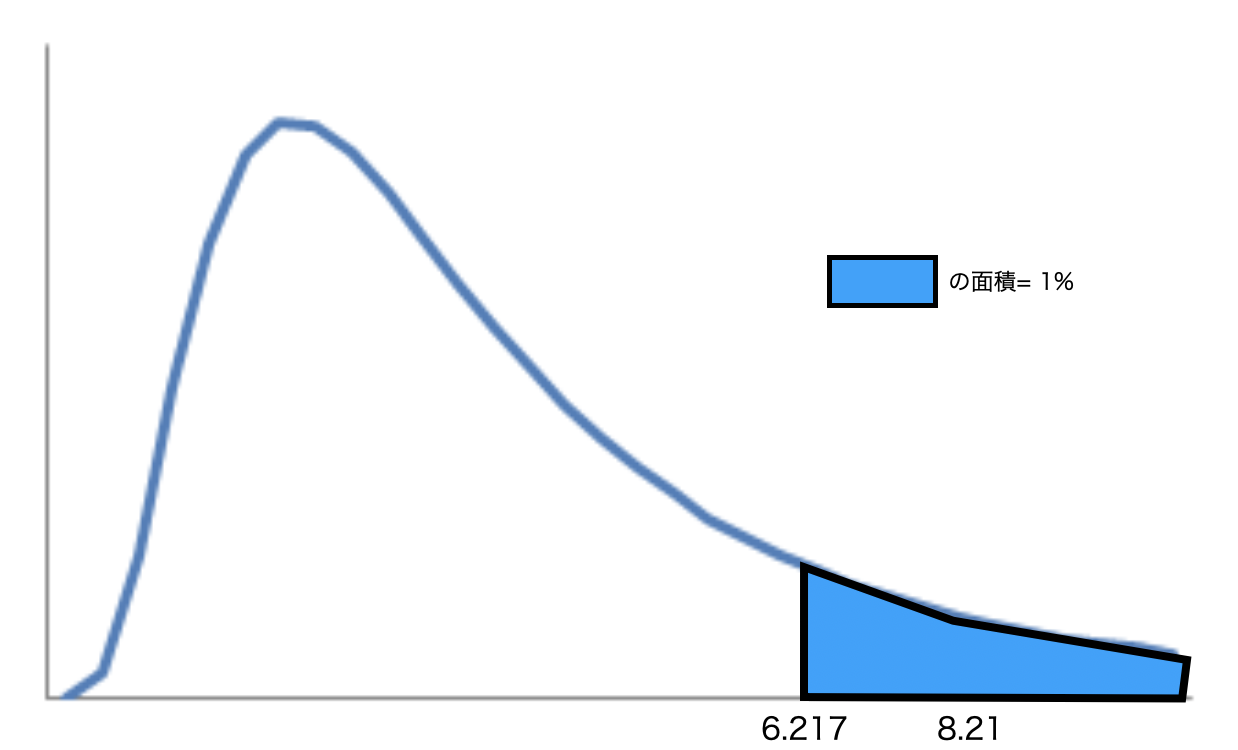
\includegraphics[width=10cm]{../pics/f.png}
  \caption{F検定}
  \label{fig:f}
\end{figure}

\newpage

\section{式変形の証明}
\subsection{$\delta$関数と基本統計量}
式変形で用いる, $\delta$関数を定義し, その他統計量を導く. 
まず, 式\eqref{eq:delta_func}を$\delta$関数と定義する. 
\begin{align}
  \label{eq:delta_func}
  \delta (j, l)
  &= \left\{
  \begin{array}{ll}
    1 &(j=l) \\
    0 &(j\neq l)
  \end{array}
  \right.
\end{align}
ここで, $\bm{V}=[s_{jl}]$と$\bm{V}^{-1}=[s^{jl}]$と$p$次単位行列$\bm{I}$について
\begin{align*}
  \bm{V}^{-1}\bm{V} = \bm{VV}^{-1} = \bm{I}
\end{align*}
すなわち
\begin{align*}
  \left[
    \begin{array}{cccccc}
      s^{11} &s^{12} & \cdots &s^{1l} &\cdots &s^{1p} \\
      s^{21} &s^{22} & \cdots &s^{2l} &\cdots &s^{2p} \\
      \vdots &\vdots & \ddots &\vdots &\ddots &\vdots \\
      s^{j1} &s^{j2} & \cdots &s^{jl} &\cdots &s^{jp} \\
      \vdots &\vdots & \ddots &\vdots &\ddots &\vdots \\
      s^{p1} &s^{p2} & \cdots &s^{pl} &\cdots &s^{pp} 
    \end{array}
  \right]
  \left[
    \begin{array}{cccccc}
      s_{11} &s_{12} & \cdots &s_{1l} &\cdots &s_{1p} \\
      s_{21} &s_{22} & \cdots &s_{2l} &\cdots &s_{2p} \\
      \vdots &\vdots & \ddots &\vdots &\ddots &\vdots \\
      s_{j1} &s_{j2} & \cdots &s_{jl} &\cdots &s_{jp} \\
      \vdots &\vdots & \ddots &\vdots &\ddots &\vdots \\
      s_{p1} &s_{p2} & \cdots &s_{pl} &\cdots &s_{pp} 
    \end{array}
  \right]
  =
  \left[
    \begin{array}{cccc}
      1 &0 &\cdots &0 \\
      0 &1 &\cdots &\vdots \\
      \vdots &\vdots &\ddots &\vdots \\
      0 &0 &\cdots &1
    \end{array}
  \right]
\end{align*}
行番号と列番号が一致するときにのみ1をとることから, 
\begin{align}
  \label{eq:sum_delta}
  \sum_{m=1}^ps^{jm}s_{ml} = \sum_{m=1}^ps_{ml}s^{jm}=\delta(j, l)
\end{align}
となる. また, 定数$b_j, j=1, 2, \cdots, p$について, 
\begin{align}
  \label{eq:sum_delta_constant}
  \sum_{l=1}^pb_l\delta (j, l)=b_j
\end{align}
が成り立つ. \\

$y_i$の期待値$\operatorname{E}(y_i)$は
\begin{align}
  \notag
  \operatorname{E}(y_i)
  &= \operatorname{E}(a_0 + a_1x_{1i}+ \cdots + a_px_{pi}+e_i) 
  \text{\quad ($\because$ 式\eqref{eq:model} 
  \;$y_i = a_0 + a_1x_{1i} + \cdots + a_px_{pi}+e_i$より)}\\
  \notag
  &= a_0 + a_1x_{1i} + \cdots + a_px_{pi} + \operatorname{E}(e_i) \\
  \label{eq:e_yi} 
  &= a_0 + a_1x_{1i} + \cdots + a_px_{pi} 
  \text{\quad ($\because \; \operatorname{E}(e_i) = 0$)}
\end{align}

$y_i, y_k$の共分散$\operatorname{Cov}(y_i, y_k)$は, 
\begin{align}
  \notag
  \operatorname{Cov}(y_i, y_k)
  &= \operatorname{E}\left[\{y_i-\operatorname{E}(y_i)\}\{y_k-\operatorname{E}(y_k)\}\right] \\
  \notag
  &=\operatorname{E}\left[\{y_i-(a_0 + a_1x_{1i} + \cdots + a_px_{pi})\}\{y_k-(a_0 + a_1x_{1k} + \cdots + a_px_{pk})\}\right] \\
  \notag
  &\text{\quad ($\because$式\eqref{eq:e_yi}\; $\operatorname{E}(y_i)=a_0 + a_1x_{1i} + \cdots + a_px_{pi} $より)} \\
  \notag
  &= \operatorname{E}(e_ie_k) \\
  \notag
  &= \operatorname{E}\left[\{e_i-\operatorname{E}(e_i)\}\{e_k-\operatorname{E}(e_k)\}\right] \text{\;\;\; ($\because \operatorname{E}(e_i)=0$より)} \\
  \label{eq:cov_yiyk}
  &= \operatorname{Cov}(e_i, e_k)
\end{align}
$\operatorname{Cov}(e_i, e_k)$について, $e_i, e_k$は互いに独立で無相関であるため, 
\begin{align*}
  \left\{
    \begin{array}{ll}
      \operatorname{Cov}(e_i, e_k) =0 &(i\neq k) \\
      \operatorname{Cov}(e_i, e_k) =\operatorname{V}(e_i) &(i= k) 
    \end{array}
  \right.
\end{align*}
となる. また, 定数$c_i, i=1, 2, \cdots, n$に関して, 
\begin{align}
  \label{eq:sum_cov}
  \sum_{k=1}^nc_k\operatorname{Cov}(e_i, e_k) = c_i\operatorname{V}(e_i) =c_i\sigma^2
\end{align}
が成り立つ. 

そして, 共分散$s_{jl}, j, l=1, 2, \cdots, p$について, 
\begin{align}
  \label{eq:cov_jl_2}
  s_{jl} = \frac{1}{n}\sum_{i=1}^n(x_{ji}-\bar{x}_j)(x_{li}-\bar{x}_l) = \frac{1}{n}\sum_{i=1}^nx_{ji}x_{li}-\bar{x}_j\bar{x}_l
\end{align}
が成り立つ. 

\subsection{式\eqref{eq:regre_3}の導出}
\label{sec:6siki}
式\eqref{eq:regre_3}を導出するにあたって再掲する. 
\begin{alignat*}{2}
  &\operatorname{E}(\hat{a}_j) = a_j, &  &j=1, 2, \cdots, p \tag{\ref{eq:e_j}}\\
  %\label{eq:v_j}
  &\operatorname{V}(\hat{a}_j) = \frac{s^{jj}\sigma^2}{n},& &j=1, 2, \cdots, p \tag{\ref{eq:v_j}}\\
  %\label{eq:cov_jl}
  &\operatorname{Cov}(\hat{a}_j, \hat{a}_l) =\frac{s^{jl}\sigma^2}{n},& &j\neq l,\; j, l=1, 2, \cdots, p \tag{\ref{eq:cov_jl}}\\
  %\label{eq:e_0}
  &\operatorname{E}(\hat{a}_0)=a_0 \tag{\ref{eq:e_0}}\\
  %\label{eq:v_0}
  &\operatorname{V}(\hat{a}_0) = \left(\frac{1}{n}+\sum_{j=1}^p\sum_{l=1}^p\frac{\bar{x}_j\bar{x}_ls^{jl}}{n}\right)\sigma^2 \tag{\ref{eq:v_0}}\\
  %\label{eq:cov_0j}
  &\operatorname{Cov}(\hat{a}_0, \hat{a}_j) = -\sum_{l=1}^p\frac{\bar{x}_ls^{jl}\sigma^2}{n},&\quad & j=1, 2, \cdots, p \tag{\ref{eq:cov_0j}}
\end{alignat*}

\subsubsection{式\eqref{eq:e_j} $\operatorname{E}(\hat{a}_j) = a_j$の導出}

%期待値E(\hat{a}_j)

\begin{align*}
  \operatorname{E}(\hat{a}_j) 
  &= \operatorname{E}\left\{
      \frac{1}{n}\sum_{i=1}^n\sum_{l=1}^ps^{jl}(x_{li}-\bar{x}_l)y_i
    \right\} 
    \text{\quad ($\because$ 式\eqref{eq:j_regressionC}\; $\hat{a}_j= \frac{1}{n}\sum_{l=1}^p\sum_{i=1}^ns^{jl}(x_{li}-\bar{x}_l)y_i$より)}\\
  &=\frac{1}{n}\sum_{i=1}^n\sum_{l=1}^ps^{jl}(x_{li}-\bar{x}_l)\operatorname{E}(y_i) \\
  &=\frac{1}{n}\sum_{i=1}^n\sum_{l=1}^ps^{jl}(x_{li}-\bar{x}_l)(a_0 + a_1x_{1i} + \cdots + a_px_{pi}) \\
  &\text{\quad ($\because$式\eqref{eq:e_yi}\; $\operatorname{E}(y_i)=a_0 + a_1x_{1i} + \cdots + a_px_{pi} $より)} \\
  &= \frac{1}{n}\sum_{i=1}^n\sum_{l=1}^ps^{jl}(x_{li}-\bar{x}_l)
  \left(
    a_0+\sum_{j'=1}^pa_{j'}x_{j'i}
  \right) \\
  &= \frac{1}{n}\sum_{l=1}^ps^{jl}
  \left\{
    a_0\sum_{i=1}^n(x_{li}-\bar{x}_l)
    +\sum_{j'=1}^pa_{j'}\sum_{i=1}^n(x_{li}-\bar{x}_l)x_{j'i}
  \right\} \\
  &=\frac{1}{n}\sum_{l=1}^ps^{jl}\sum_{j'=1}^pa_{j'}\sum_{i=1}^n(x_{li}x_{j'i}-\bar{x}_lx_{j'i}) \\
  &= \frac{1}{n}\sum_{l=1}^ps^{jl}\sum_{j'=1}^pa_{j'}
  \left(
    \sum_{i=1}^nx_{li}x_{j'i}
    -\bar{x}_l\sum_{i=1}^nx_{j'i}
  \right) \\
  &= \sum_{l=1}^ps^{jl}\sum_{j'=1}^pa_{j'}
  \left(
    \frac{1}{n}\sum_{i=1}^nx_{li}x_{j'i}
    -\bar{x}_l\bar{x}_{j'}
  \right) \\
  &= \sum_{l=1}^ps^{jl}\sum_{j'=1}^pa_{j'}s_{lj'} 
  \text{\quad ($\because$ 式\eqref{eq:cov_jl_2} \;$s_{jl} = \frac{1}{n}\sum_{i=1}^nx_{ji}x_{li}-\bar{x}_j\bar{x}_l$より)} \\
  &= \sum_{j'=1}^pa_{j'}\sum_{l=1}^ps^{jl}s_{lj'} \\
  &= \sum_{j'=1}^pa_{j'}\delta(j, j') 
  \text{\quad ($\because$ 式\eqref{eq:sum_delta} $\sum_{m=1}^ps^{jm}s_{ml} =\delta(j, l)$より)}\\
  &=a_j 
  \text{\quad ($\because$ 式\eqref{eq:sum_delta_constant} \;$\sum_{l=1}^pb_l\delta (j, l)=b_j$より)}
\end{align*}

\subsubsection{式\eqref{eq:cov_jl}\; $\operatorname{Cov}(\hat{a}_j, \hat{a}_l) =\frac{s^{jl}\sigma^2}{n}$の導出}

%共分散Cov(\hat{a}_j, \hat{a}_l)

\begin{align*}
  \operatorname{Cov}(\hat{a}_j, \hat{a}_l)
  &= \operatorname{E}\left[
    \left\{
      \hat{a}_j-\operatorname{E}(\hat{a}_j)
    \right\}
    \left\{
      \hat{a}_l-\operatorname{E}(\hat{a}_l)
    \right\}
  \right] \\
  \begin{split}
  &= \operatorname{E}\left[
    \left\{
      \frac{1}{n}\sum_{i=1}^n\sum_{j'=1}^ps^{jj'}(x_{j'i}-\bar{x}_{j'})y_i
      -\operatorname{E}\left(
        \frac{1}{n}\sum_{i=1}^n\sum_{j'=1}^ps^{jj'}(x_{j'i}-\bar{x}_{j'})y_i
      \right)
    \right\} 
    \right.\\
  &\quad \left.
    \left\{
      \frac{1}{n}\sum_{k=1}^n\sum_{l'=1}^ps^{ll'}(x_{l'k}
      -\bar{x}_{l'})y_k-\operatorname{E}\left(
        \frac{1}{n}\sum_{k=1}^n\sum_{l'=1}^ps^{ll'}(x_{l'k}-\bar{x}_{l'})y_k
      \right)
    \right\}
  \right] 
  \end{split} \\
  & \text{\quad ($\because$ 式\eqref{eq:j_regressionC}\; $\hat{a}_j= \frac{1}{n}\sum_{l=1}^p\sum_{i=1}^ns^{jl}(x_{li}-\bar{x}_l)y_i$より)} \\
  &= \operatorname{E}\left[
    \left\{
      \frac{1}{n}\sum_{i=1}^n\sum_{j'=1}^ps^{jj'}
      (x_{j'i}-\bar{x}_{j'})
      \left(
        y_i-\operatorname{E}(y_i)
      \right)
    \right\}
    \left\{
      \frac{1}{n}\sum_{k=1}^n\sum_{l'=1}^ps^{ll'}
      (x_{l'k}-\bar{x}_{l'})
      \left(
        y_k-\operatorname{E}(y_k)
      \right)
    \right\}
  \right] \\
  &= \operatorname{E}\left[
    \frac{1}{n^2}\sum_{j'=1}^p\sum_{l'=1}^ps^{jj'}s^{ll'}
    \sum_{i=1}^n\sum_{k=1}^n
    (x_{j'i}-\bar{x}_{j'})(x_{l'k}-\bar{x}_{l'})
    \left\{
      y_i-\operatorname{E}(y_i)
    \right\}
    \left\{
      y_k-\operatorname{E}(y_k)
    \right\}
  \right] \\
  &= \frac{1}{n^2}\sum_{j'=1}^p\sum_{l'=1}^ps^{jj'}s^{ll'}
  \sum_{i=1}^n\sum_{k=1}^n
  (x_{j'i}-\bar{x}_{j'})(x_{l'k}-\bar{x}_{l'})
  \operatorname{E}\left[
    \left\{
      y_i-\operatorname{E}(y_i)
    \right\}
    \left\{
      y_k-\operatorname{E}(y_k)
    \right\}
  \right] \\
  &= \frac{1}{n^2}\sum_{j'=1}^p\sum_{l'=1}^ps^{jj'}s^{ll'}
  \sum_{i=1}^n\sum_{k=1}^n
  (x_{j'i}-\bar{x}_{j'})(x_{l'k}-\bar{x}_{l'})\operatorname{Cov}(y_i, y_k) \\
  &= \frac{1}{n^2}\sum_{j'=1}^p\sum_{l'=1}^ps^{jj'}s^{ll'}
  \sum_{i=1}^n\sum_{k=1}^n
  (x_{j'i}-\bar{x}_{j'})(x_{l'k}-\bar{x}_{l'})\operatorname{Cov}(e_i, e_k) \\
  & \text{\quad ($\because$ 式\eqref{eq:cov_yiyk}\; $\operatorname{Cov}(y_i, y_k)= \operatorname{Cov}(e_i, e_k)$より)} \\
  &= \frac{1}{n}\sum_{j'=1}^p\sum_{l'=1}^ps^{jj'}s^{ll'}
  \frac{1}{n}\sum_{i=1}^n
  (x_{j'i}-\bar{x}_{j'})(x_{l'i}-\bar{x}_{l'})\sigma^2 \\
  & \text{\quad ($\because$ 式\eqref{eq:sum_cov}
  \; $\sum_{k=1}^nc_k\operatorname{Cov}(e_i, e_k) = c_i\operatorname{V}(e_i) =c_i\sigma^2$より)} \\
  &= \frac{1}{n}\sum_{j'=1}^p\sum_{l'=1}^p
  s^{jj'}s^{ll'}s_{j'l'}\sigma^2 \\
  &= \frac{\sigma^2}{n}\sum_{l'=1}^ps^{ll'}
  \sum_{j'=1}^ps^{jj'}s_{j'l'} \\
  &= \frac{\sigma^2}{n}\sum_{l'=1}^ps^{ll'}\delta(j, l') \text{\;\;\; ($\because$ 式\eqref{eq:sum_delta}$\sum_{m=1}^ps^{jm}s_{ml} = \sum_{m=1}^ps_{ml}s^{jm}=\delta(j, l)$より)} \\
  &= \frac{s^{lj}\sigma^2}{n} = \frac{s^{jl}\sigma^2}{n}
  \text{\quad ($\because$ 式\eqref{eq:sum_delta_constant} \;$\sum_{l=1}^pb_l\delta (j, l)=b_j$より)}
\end{align*}
\qed

\subsubsection{式\eqref{eq:v_j}\; $\operatorname{V}(\hat{a}_j) = \frac{s^{jj}\sigma^2}{n}$の導出}

%分散V(\hat{a}_j)

式\eqref{eq:cov_jl}において, $j, l$が$j=l$のときであるから, 
\begin{align*}
  \operatorname{V}(\hat{a}_j) = \operatorname{Cov}(\hat{a}_j, \hat{a}_j) = \frac{s^{jj}\sigma^2}{n}
\end{align*}
\qed

\subsubsection{式\eqref{eq:e_0}\; $\operatorname{E}(\hat{a}_0)=a_0$の導出}

%期待値E(\hat{a}_0)

\begin{align*}
  \operatorname{E}(\hat{a}_0)
  &= \operatorname{E}(\bar{y}-\hat{a}_1\bar{x}_1-\cdots -\hat{a}_p\bar{x}_p) \\
  &= \operatorname{E}(\bar{y})
  - \operatorname{E}\left(
    \sum_{j=1}^p\hat{a}_j\bar{x}_j
  \right) \\
  &= \operatorname{E}\left(
    \frac{1}{n}\sum_{i=1}^ny_i
  \right)
  -\sum_{j=1}^p\operatorname{E}(\hat{a}_j)\bar{x}_j \\
  &= \frac{1}{n}\sum_{i=1}^n\operatorname{E}(y_i)
  -\sum_{j=1}^pa_j\bar{x}_j 
  \text{\quad ($\because$ 式\eqref{eq:e_j}より\; $\operatorname{E}(\hat{a}_j)=a_j$)} \\
  &= \frac{1}{n}\sum_{i=1}^n(a_0 + a_1x_{1i} 
  + \cdots + a_px_{pi})-\sum_{j=1}^pa_j\bar{x}_j \\
  &\text{\quad ($\because$ 式\eqref{eq:e_yi} \;$\operatorname{E}(y_i)=a_0 + a_1x_{1i} + \cdots + a_px_{pi}$より)}\\
  &= \frac{1}{n}\sum_{i=1}^n\left(
    a_0 + \sum_{j=1}^pa_jx_{ji}
  \right)  
  -\sum_{j=1}^pa_j\bar{x}_j\\
  &=\frac{1}{n}\sum_{i=1}^na_0
  +\sum_{j=1}^pa_j\frac{1}{n}\sum_{i=1}^nx_{ji}-\sum_{j=1}^pa_j\bar{x}_j \\
  &= a_0 + \sum_{j=1}^pa_j\bar{x}_j - \sum_{j=1}^pa_j\bar{x}_j \\
  &= a_0 
\end{align*}
\qed

\subsubsection{式\eqref{eq:v_0}\; $\operatorname{V}(\hat{a}_0) = \left(\frac{1}{n}+\sum_{j=1}^p\sum_{l=1}^p\frac{\bar{x}_j\bar{x}_ls^{jl}}{n}\right)\sigma^2$の導出}

%分散V(\hat{a}_0)

\begin{align}
  \notag %1
  \operatorname{V}(\hat{a}_0)
  &=\operatorname{E}\left[
    (\hat{a}_0-\operatorname{E}(\hat{a}_0))^2
  \right] \\
  \notag %2
  &= \operatorname{E}\left[
    \left\{
      \bar{y}-(\hat{a}_1\bar{x}_1+ \cdots + \hat{a}_p\bar{x}_p)-\operatorname{E}\left(\bar{y}-(\hat{a}_1\bar{x}_1+\cdots + \hat{a}_p\bar{x}_p)\right)
    \right\}^2
  \right] \\
  \notag
  &\text{\quad ($\because$ 式\eqref{eq:sec5_y_bar}
  \; $\hat{a}_0 = \bar{y}-(\hat{a}_1\bar{x}_1+\cdots+\hat{a}_p\bar{x}_p)$より)} \\
  \notag %3
  &= \operatorname{E}\left[
    \left\{
      \bar{y}-(\hat{a}_1\bar{x}_1+ \cdots + \hat{a}_p\bar{x}_p)-
      \left(\operatorname{E}(\bar{y})-\operatorname{E}(\hat{a}_1\bar{x}_1+\cdots + \hat{a}_p\bar{x}_p)\right)
    \right\}^2
  \right]\\
  \notag %4
  &= \operatorname{E}\left[
    \left\{
      (\bar{y}-\operatorname{E}(\bar{y}))-\left(\sum_{j=1}^p\hat{a}_j\bar{x}_j-\sum_{j=1}^p\operatorname{E}(\hat{a}_j\bar{x}_j)\right)
    \right\}^2
  \right]\\
  \notag %5
  \begin{split}
    &= \operatorname{E}[\{\bar{y}-\operatorname{E}(\bar{y})\}^2]
    +\operatorname{E}\left[
    \left\{
      \sum_{j=1}^p\hat{a}_j\bar{x}_j-\sum_{j=1}^p\operatorname{E}(\hat{a}_j\bar{x}_j)
    \right\}^2
  \right] \\
  & \quad -2\operatorname{E}\left[
    \{\bar{y}-\operatorname{E}(\bar{y})\}
    \left\{
      \sum_{j=1}^p\hat{a}_j\bar{x}_j-\sum_{j=1}^p\operatorname{E}(\hat{a}_j\bar{x}_j)
    \right\}
  \right]
  \end{split}\\
  \notag %6
  &= \operatorname{V}(\bar{y}) 
  + \operatorname{E}\left[
    \left\{
      \sum_{j=1}^p\bar{x}_j(\hat{a}_j-\operatorname{E}(\hat{a}_j))
    \right\}^2
  \right] 
  -2\operatorname{E}\left[
    \{\bar{y}-\operatorname{E}(\bar{y})\}\sum_{j=1}^p\bar{x}_j\{\hat{a}_j-\operatorname{E}(\hat{a}_j)\}
  \right] \\
  \notag %7
  &= \operatorname{V}(\bar{y})
  + \operatorname{E}\left[
    \left\{
      \sum_{j=1}^p\bar{x}_j(\hat{a}_j-\operatorname{E}(\hat{a}_j))
    \right\}
    \left\{
      \sum_{l=1}^p\bar{x}_l(\hat{a}_l-\operatorname{E}(\hat{a}_l))
    \right\}
  \right] 
  - 2\sum_{j=1}^p\bar{x}_j\operatorname{E}\left[
    \{\bar{y}-\operatorname{E}(\bar{y})\}\{\hat{a}_j-\operatorname{E}(\hat{a}_j)\}
  \right]\\
  \label{eq:v_y_transform} %8
  &= \operatorname{V}(\bar{y}) 
  +\sum_{j=1}^p\sum_{l=1}^p\bar{x}_j\bar{x}_l\operatorname{Cov}(\hat{a}_j, \hat{a}_l)
  - 2\sum_{j=1}^p\bar{x}_j\operatorname{Cov}(\bar{y}, \hat{a}_j)
\end{align}
ここで式\eqref{eq:v_y_transform}の第1項について, 
\begin{align}
  \notag %1
  \operatorname{V}(\bar{y})
  &= \operatorname{V}\left(
    \frac{1}{n}\sum_{i=1}^ny_i
  \right)\\
  \notag %2
  &=\operatorname{V}\left(
    \frac{1}{n}\sum_{i=1}^n(a_0+a_1x_{1i}+\cdots +a_px_{pi}+e_i
  )\right) \\
  \notag %3
  &= \operatorname{V}\left(\frac{1}{n}\sum_{i=1}^ne_i\right) \\
  \notag %4
  &= \frac{1}{n^2}\sum_{i=1}^n\operatorname{V}(e_i) \\
  \notag %5
  &= \frac{1}{n^2}\sum_{i=1}^n\sigma^2 \\
  \label{eq:v_y_bar} %6
  &= \frac{1}{n^2}n\sigma^2 = \frac{\sigma^2}{n}
\end{align}
次に式\eqref{eq:v_y_transform}の第3項について, 
%共分散Cov(\bar{y}, \hat{a}_j)
\begin{align}
  \notag %1
  \operatorname{Cov}(\bar{y}, \hat{a}_j)
  &= \operatorname{E}\left[
    \left\{
      \bar{y}-\operatorname{E}(\bar{y})
    \right\}
    \left\{
      \hat{a}_j-\operatorname{E}(\hat{a}_j)
    \right\}
  \right]\\
  \notag %2
  \begin{split}
    &=\operatorname{E}\left[
      \left\{
        \frac{1}{n}\sum_{i=1}^ny_i - \operatorname{E}\left(
          \frac{1}{n}\sum_{i=1}^ny_i
        \right)
      \right\}
    \right. \\
    &\quad \left.
      \left\{
        \frac{1}{n}\sum_{i=1}^n\sum_{l=1}^ps^{jl}(x_{li}-\bar{x}_l)y_i
        -\operatorname{E}\left(
          \frac{1}{n}\sum_{i=1}^n\sum_{l=1}^ps^{jl}(x_{li}-\bar{x}_l)y_i
        \right)
      \right\}
    \right]
  \end{split}\\
  \notag
  &\text{\quad ($\because$ 式\eqref{eq:j_regressionC}
  \; $\hat{a}_{j}=\frac{1}{n}\sum_{l=1}^p\sum_{i=1}^ns^{jl}(x_{li}-\bar{x}_l)y_i$より)} \\
  \notag %3
  \begin{split}
    &= \operatorname{E}\left[
      \left\{
        \frac{1}{n}\sum_{i=1}^ny_i 
        - \frac{1}{n}\sum_{i=1}^n\operatorname{E}(y_i)
      \right\}
    \right. \\
    &\quad \left.
      \left\{
        \frac{1}{n}\sum_{i=1}^n\sum_{l=1}^ps^{jl}(x_{li}-\bar{x}_l)y_i
        - \frac{1}{n}\sum_{i=1}^n\sum_{l=1}^ps^{jl}(x_{li}-\bar{x}_l)
        \operatorname{E}(y_i)
      \right\}
    \right] 
  \end{split}\\
  \notag %4
  &= \operatorname{E}\left[
    \left\{
      \frac{1}{n}\sum_{i=1}^n
      \left(
        y_i - \operatorname{E}(y_i)
      \right)
    \right\}
    \left\{
      \frac{1}{n}\sum_{i=1}^n\sum_{l=1}^ps^{jl}(x_{li}-\bar{x}_{l})
      \left(
        y_i - \operatorname{E}(y_i)
      \right)
    \right\}
  \right] \\
  \notag %5
  &= \frac{1}{n}\sum_{l=1}^ps^{jl}
  \frac{1}{n}\sum_{i=1}^n(x_{li}-\bar{x}_{l})\operatorname{E}\left[
    \left\{
      y_i-\operatorname{E}(y_i)
    \right\}^2
  \right]\\
  \label{eq:cov_y_bar_a_hat}
  &=0
\end{align}
式\eqref{eq:v_y_bar}と式\eqref{eq:cov_y_bar_a_hat}を式\eqref{eq:v_y_transform}に代入すると, 
\begin{align*}
  \operatorname{V}(\hat{a}_0)
  &= \operatorname{V}(\bar{y}) 
  + \sum_{j=1}^p\sum_{l=1}^p\bar{x}_j\bar{x}_l\operatorname{Cov}(\hat{a}_j, \hat{a}_l)
  -2\sum_{j=1}^p\bar{x}\operatorname{Cov}(\bar{y}, \hat{a}_j) \\
  &= \frac{\sigma^2}{n} + \sum_{j=1}^p\sum_{l=1}^p\bar{x}_j\bar{x}_l\left(
    \frac{s^{jl}\sigma^2}{n}
  \right) \text{\;\;\; ($\because$ 式\eqref{eq:cov_jl}\; $\operatorname{Cov}(\hat{a}_j, \hat{a}_l) =\frac{s^{jl}\sigma^2}{n}$より)}\\
  &= \left(\frac{1}{n}+\sum_{j=1}^p\sum_{l=1}^p\frac{\bar{x}_j\bar{x}_ls^{jl}}{n}\right)\sigma^2
\end{align*}
\qed

\subsubsection{式\eqref{eq:cov_0j}\; $\operatorname{Cov}(\hat{a}_0, \hat{a}_j) = -\sum_{l=1}^p\frac{\bar{x}_ls^{jl}\sigma^2}{n}$の導出}

%共分散Cov(\hat{a}_0, \hat{a}_j)

\begin{align*}
  \operatorname{Cov}(\hat{a}_0, \hat{a}_j)
  &= \operatorname{E}\left[
    \left\{
      \hat{a}_0-\operatorname{E}(\hat{a_0})
    \right\}
    \left\{
      \hat{a}_j-\operatorname{E}(\hat{a_j})
    \right\}
  \right] \\
  &= \operatorname{E}\left[
    \left\{
      (\bar{y}-\hat{a}_1\bar{x}_1-\cdots -\hat{a}_p\bar{x}_p)-\operatorname{E}(\bar{y})+\operatorname{E}(\hat{a}_1\bar{x}_1)+\cdots +\operatorname{E}(\hat{a}_p\bar{x}_p)
    \right\}
    \left\{
      \hat{a}_j-\operatorname{E}(\hat{a}_j) 
    \right\}
  \right] \\
  &\text{\quad ($\because$ 式\eqref{eq:sec5_y_bar} \;$\hat{a}_0=\bar{y}-(\hat{a}_1\bar{x}_1+\cdots+\hat{a}_p\bar{x}_p)$より)}\\
  \begin{split}
    &= \operatorname{E}\left[
    \left\{
      \bar{y}-\operatorname{E}(\bar{y})
    \right\}
    \left\{
      \hat{a}_j-\operatorname{E}(\hat{a}_j)
    \right\}
    \right]
    -\operatorname{E}\left[
      \bar{x}_1\{
        \hat{a}_1-\operatorname{E}(\hat{a}_1)
      \}
      \{
        \hat{a}_j-\operatorname{E}(\hat{a}_j)
      \}
    \right] \\
    &\quad - \cdots -\operatorname{E}\left[
      \bar{x}_p\{\hat{a}_p-\operatorname{E}(\hat{a}_p)\}\{\hat{a}_j-\operatorname{E}(\hat{a}_j)\}
    \right]
  \end{split} \\
  &=\operatorname{Cov}(\bar{y}, \hat{a}_j)
  -\bar{x}_1\operatorname{Cov}(\hat{a}_1, \hat{a}_j)- \cdots 
  -\bar{x}_p\operatorname{Cov}(\hat{a}_p, \hat{a}_j) \\
  &= \operatorname{Cov}(\bar{y}, \hat{a}_j) 
  -\sum_{l=1}^p\bar{x}_l\operatorname{Cov}(\hat{a}_j, \hat{a}_l)\\
  &= -\sum_{l=1}^p\frac{\bar{x}_ls^{jl}\sigma^2}{n} \\
  &\text{\; ($\because$ 式\eqref{eq:cov_y_bar_a_hat}\; 
  $\operatorname{Cov}(\bar{y}, \hat{a}_j)=0$と
  式\eqref{eq:cov_jl}$ \; 
  \operatorname{Cov}(\hat{a}_j, \hat{a}_l) =\frac{s^{jl}\sigma^2}{n}$より)}
\end{align*}
\qed

\subsection{式\eqref{eq:f_dist}\; $\operatorname{F}(\hat{a}_0, \hat{a}_1, \cdots, \hat{a}_p)= n(s_{yy}-\sum_{l=1}^ps_{yl}\hat{a}_l)$の導出}
\label{sec:mean_squared_error_sum}

%残差平方和F

\begin{align}
  \notag
  \operatorname{F}(\hat{a}_0, \hat{a}_1, \cdots, \hat{a}_p)
  &= \sum_{i=1}^p\left\{y_i-(\hat{a}_0+\hat{a}_1x_{1i}+\cdots+\hat{a}_px_{pi})\right\}^2 \\
  \notag
  &=\sum_{i=1}^n\left\{
    (y_i-\bar{y})-\hat{a}_1(x_{1i}-\bar{x}_1)-\cdots -\hat{a}_p(x_{pi}-\bar{x}_p)
  \right\}^2 \\
  \notag
  &\text{\quad ($\because$ 式\eqref{eq:sec5_y_bar} \;
  $\hat{a}_0=\bar{y}-(\hat{a}_1\bar{x}_1+\cdots+\hat{a}_p\bar{x}_p)$より)}\\
  \begin{split}
    \label{eq:f_dist_transform}
    &= \sum_{i=1}^n(y_i-\bar{y})^2
    -2\sum_{i=1}^n(y_i-\bar{y})\sum_{j=1}^p\hat{a}_j(x_{ji}-\bar{x}_j) \\
    & \quad + \sum_{i=1}^n\sum_{j=1}^p\sum_{l=1}^p\hat{a}_j(x_{ji}-\bar{x}_j)\hat{a}_l(x_{li}-\bar{x}_l)
  \end{split}  
\end{align}
ここで, 式\eqref{eq:f_dist_transform}の第1項は, 
\begin{align}
  \label{eq:sum_s_yy}
  \sum_{i=1}^n(y_i-\bar{y})^2 = ns_{yy}
\end{align}
また, 式\eqref{eq:f_dist_transform}の第2項は, 
\begin{align}
  \notag
  \sum_{i=1}^n(y_i-\bar{y})\sum_{j=1}^p\hat{a}_j(x_{ji}-\bar{x}_j)
  &=\sum_{j=1}^p\hat{a}_j\sum_{i=1}^n(y_i-\bar{y})(x_{ji}-\bar{x}_j)\\
  \label{eq:s_yj_hat_a}
  &= \sum_{j=1}^p\hat{a}_jns_{yj}
\end{align}
そして, 式\eqref{eq:f_dist_transform}の第3項は, 
\begin{align}
  \notag %1
  \sum_{i=1}^n\sum_{j=1}^p\sum_{l=1}^p\hat{a}_j(x_{ji}-\bar{x}_j)\hat{a}_l(x_{li}-\bar{x}_l)
  &= \sum_{j=1}^p\sum_{l=1}^p\hat{a}_j\hat{a}_l\sum_{i=1}^n(x_{ji}-\bar{x}_j)(x_{li}-\bar{x}_l) \\
  \notag %2
  &= \sum_{j=1}^p\sum_{l=1}^p\hat{a}_j\hat{a}_lns_{jl} \\
  \notag %3
  &=\sum_{j=1}^p\sum_{l=1}^p\hat{a}_j
  \left\{
    \frac{1}{n}\sum_{i=1}^n\sum_{l'=1}^ps^{ll'}(x_{l'i}-\bar{x}_{l'})y_i
  \right\}ns_{jl} \\
  \notag %4
  & \text{\quad ($\because$ 式\eqref{eq:j_regressionC}
  \; $\hat{a}_{j} =\frac{1}{n}\sum_{l=1}^p\sum_{i=1}^ns^{jl}(x_{li}-\bar{x}_l)y_i$より)} \\
  \notag %5
  &= \sum_{j=1}^p\hat{a}_j\sum_{i=1}^ny_i\sum_{l'=1}^p(x_{l'i}-\bar{x}_{l'})\sum_{l=1}^ps_{jl}s^{ll'} \\
  \notag %6
  &=\sum_{j=1}^p\hat{a}_j\sum_{i=1}^ny_i\sum_{l'=1}^p(x_{l'i}-\bar{x}_{l'})\delta(j, l') \\
  \notag %7
  & \text{\quad ($\because$ 式\eqref{eq:sum_delta}
  \; $\sum_{m=1}^ps_{ml}s^{jm}=\delta(j, l)$より)}\\
  \notag %8
  &=\sum_{j=1}^p\hat{a}_j\sum_{i=1}^n(x_{ji}-\bar{x}_j)y_i \\
  \notag %9
  &\text{\quad ($\because$ 式\eqref{eq:sum_delta_constant}
  \; $\sum_{l=1}^pb_l\delta (j, l)=b_j$より)} \\
  \notag
  &= \sum_{j=1}^p\hat{a}_j\sum_{i=1}^n(x_{ji}-\bar{x}_j)
  \{
    (y_i-\bar{y})+\bar{y}
  \} \\
  \notag %10
  &=\sum_{j=1}^p\hat{a}_j\left\{
    \sum_{i=1}^n(x_{ji}-\bar{x}_j)(y_i-\bar{y})
    + \bar{y}\sum_{i=1}^n(x_{ji}-\bar{x}_j)
  \right\}\\
  \label{eq:hat_a_n_s_yj} %11
  &=\sum_{j=1}^p\hat{a}_jns_{yj}
\end{align}
式\eqref{eq:f_dist_transform}に式\eqref{eq:sum_s_yy}, 式\eqref{eq:s_yj_hat_a}, 式\eqref{eq:hat_a_n_s_yj}を代入すると, 
\begin{align*}
  \operatorname{F}(\hat{a}_0, \hat{a}_1, \cdots, \hat{a}_p) 
  &= \sum_{i=1}^n(y_i-\bar{y})^2
  -2\sum_{i=1}^n(y_i-\bar{y})\sum_{j=1}^p\hat{a}_j(x_{ji}-\bar{x}_j) \\
  & \quad + \sum_{i=1}^n\sum_{j=1}^p\sum_{l=1}^p\hat{a}_j(x_{ji}-\bar{x}_j)\hat{a}_l(x_{li}-\bar{x}_l) \\
  &= ns_{yy} -2\sum_{j=1}^p\hat{a}_jns_{yj}+\sum_{j=1}^p\hat{a}_jns_{yj} \\
  &= n\left(
    s_{yy}-\sum_{j=1}^p\hat{a}_js_{yj}
  \right)
\end{align*}
\qed

\subsection{$\operatorname{V}_e$が誤差分散$\sigma^2$の不偏推定値であることの証明}
\label{sec:ve_unbiased}
式\eqref{eq:unbiasedV}\; $\operatorname{V}_e = \frac{\operatorname{F}(\hat{a}_0, \hat{a}_1, \cdots, \hat{a}_p)}{n-p-1}$が誤差分散$\sigma^2$の不偏推定値であることを示すため, $\operatorname{F}(\hat{a}_0, \hat{a}_1, \cdots, \hat{a}_p)$の期待値を求める. 

\begin{align}
  \notag %1
  \operatorname{E}\left[\operatorname{F}(\hat{a}_0, \hat{a}_1, \cdots, \hat{a}_p)
  \right]
  &= \operatorname{E}\left[
    \sum_{i=1}^n
    \left\{
      y_i-(\hat{a}_0+\hat{a}_1x_{1i}+\cdots +\hat{a}_px_{pi})
    \right\}^2
  \right] \\
  \notag %2
  &= \operatorname{E}\left[
    \sum_{i=1}^n
    \left\{
      (a_0-\hat{a}_0)+(a_1-\hat{a}_1)x_{1i}+\cdots +(a_p-\hat{a}_p)x_{pi}+e_i
    \right\}^2
  \right] \\
  \notag 
  & \text{\;\;\; ($\because$ 式\eqref{eq:model}
  \; $y_i = a_0 + a_1x_{1i} + \cdots + a_px_{pi}+e_i$より)} \\
  \notag %3
  \begin{split}
    &=\operatorname{E}\left[
      \sum_{i=1}^n\left\{
        (a_0-\hat{a}_0)+(a_1-\hat{a}_1)x_{1i}+\cdots +(a_p-\hat{a}_p)x_{pi}
      \right\}^2
    \right] \\
    &\quad +2\operatorname{E}\left[
      \sum_{i=1}^ne_i
      \left\{
        (a_0-\hat{a}_0)+(a_1-\hat{a}_1)x_{1i}+\cdots +(a_p-\hat{a}_p)x_{pi}
      \right\}
    \right]
    +\operatorname{E}\left(
      \sum_{i=1}^ne_i^2
    \right) 
  \end{split} \\
  \notag %3
  \begin{split}
    &=\operatorname{E}\left[
      \sum_{i=1}^n\left\{
        (a_0-\hat{a}_0)^2+2(a_0-\hat{a}_0)
        \sum_{j=1}^p(a_j-\hat{a}_j)x_{ji}
        +\sum_{j=1}^p(a_j-\hat{a}_j)x_{ji} \sum_{l=1}^p(a_l-\hat{a}_l)x_{li}
      \right\}
    \right] \\
    &\quad +2\sum_{i=1}^n\operatorname{E}\left[
      e_i(a_0-\hat{a}_0)+e_i\sum_{j=1}^p(a_j-\hat{a}_j)x_{ji}
    \right]
    +\operatorname{E}\left(
      \sum_{i=1}^ne_i^2
    \right) 
  \end{split}\\
  \notag %4
  \begin{split}
    &= \sum_{i=1}^n\operatorname{E}\left[
      \left\{
        \hat{a}_0-\operatorname{E}(\hat{a}_0)
      \right\}^2
    \right]
    +2\sum_{i=1}^n\sum_{j=1}^p\operatorname{E}\left[
      \hat{a}_0-\operatorname{E}(\hat{a}_0)
    \right]
    \operatorname{E}\left[
      \left\{
        \hat{a}_j-\operatorname{E}(\hat{a}_j)
      \right\}x_{ji}
    \right]\\
    &\quad +\sum_{i=1}^n\sum_{j=1}^p\sum_{l=1}^p\operatorname{E}\left[
      \left\{
        \hat{a}_j-\operatorname{E}(\hat{a}_j)
      \right\}
      \left\{
        \hat{a}_l-\operatorname{E}(\hat{a}_l)
      \right\}x_{ji}x_{li}
    \right] \\
    &\quad -2\sum_{i=1}^n\operatorname{E}\left[
      \left\{
        e_i-\operatorname{E}(e_i)
      \right\}
      \left\{
        \hat{a}_0-\operatorname{E}(\hat{a}_0)
      \right\}
    \right] \\
    &\quad -2\sum_{i=1}^n\sum_{j=1}^p\operatorname{E}\left[
      \left\{
        e_i-\operatorname{E}(e_i)
      \right\}
      \left\{
        \hat{a}_j-\operatorname{E}(\hat{a}_j)
      \right\}x_{ji}
    \right]
    +\operatorname{E}\left(
      \sum_{i=1}^ne_i^2
    \right) \\
    \notag
    &\text{\quad ($\because$ 式\eqref{eq:e_j}
    \; $\operatorname{E}(\hat{a}_j) = a_j$と
    式\eqref{eq:e_0}
    \; $\operatorname{E}(\hat{a}_0) = a_0$より)}
  \end{split} \\
  \label{eq:e_F_transform} %5
  \begin{split}
    &=\sum_{i=1}^n\operatorname{V}(\hat{a}_0)
    +2\sum_{i=1}^n\sum_{j=1}^p\operatorname{Cov}(\hat{a}_0, \hat{a}_j)x_{ji} 
    +\sum_{i=1}^n\sum_{j=1}^p\sum_{l=1}^p\operatorname{Cov}(\hat{a}_j, \hat{a}_l)x_{ji}x_{li} \\
    &\quad -2\sum_{i=1}^n\operatorname{Cov}(e_i, \hat{a}_0)
    -2\sum_{i=1}^n\sum_{j=1}^p\operatorname{Cov}(e_i, \hat{a}_j)x_{ji}
    +\operatorname{E}\left(
      \sum_{i=1}^ne_i^2
    \right)
  \end{split} 
\end{align}
ここで, 式\eqref{eq:e_F_transform}の第4項に関して, 
\begin{align}
  \notag %1
  \operatorname{Cov}(e_i, \hat{a}_0)
  &= \operatorname{E}\left[
    \left\{
      e_i-\operatorname{E}(e_i)
    \right\}
    \left\{
      \hat{a}_0-\operatorname{E}(\hat{a}_0)
    \right\}
  \right] \\
  \notag %2
  \begin{split}
    &= \operatorname{E}\left[
      \left\{
        e_i-\operatorname{E}(e_i)
      \right\}
    \right. \\
    &\; \left.
      \left\{
        \sum_{k=1}^n\frac{1-\sum_{j=1}^p\sum_{l=1}^p
        s^{jl}(x_{lk}-\bar{x}_l)\bar{x}_j}{n}y_k
        -\operatorname{E}\left(
          \sum_{k=1}^n\frac{1-\sum_{j=1}^p\sum_{l=1}^p
          s^{jl}(x_{lk}-\bar{x}_l)\bar{x}_j}{n}y_k
        \right)
      \right\}
    \right]
  \end{split}\\
  \notag %3
  &\text{\;\;\; ($\because$ 式\eqref{eq:0_regressionC}\; $\hat{a}_0=\frac{1}{n}\sum_{i=1}^n\left\{1-\sum_{j=1}^p\sum_{l=1}^p\bar{x}_js^{jl}(x_{li}-\bar{x}_l)\right\}y_i$)} \\
  \notag %4
  &=\operatorname{E}\left[
    \left\{
      e_i-\operatorname{E}(e_i)
    \right\}
    \sum_{k=1}^n\frac{1-\sum_{j=1}^p\sum_{l=1}^ps^{jl}(x_{lk}-\bar{x}_l)\bar{x}_j}{n}\left\{
      y_k-\operatorname{E}(y_k)
    \right\}
  \right] \\
  \notag %5
  &=\sum_{k=1}^n\frac{1-\sum_{j=1}^p\sum_{l=1}^ps^{jl}(x_{lk}-\bar{x}_l)\bar{x}_j}{n}\operatorname{E}\left[
    \left\{
      e_i-\operatorname{E}(e_i)
    \right\}
    \left\{
      y_k-\operatorname{E}(y_k)
    \right\}
  \right]\\
  \notag %6
  &=\sum_{k=1}^n\frac{1-\sum_{j=1}^p\sum_{l=1}^ps^{jl}(x_{lk}-\bar{x}_l)\bar{x}_j}{n}\operatorname{E}\left[
    \left\{
      e_i-\operatorname{E}(e_i)
    \right\}
    \left\{
      e_k-\operatorname{E}(e_k)
    \right\}
  \right] \\
  \notag 
  &\text{\quad ($\because$ 式\eqref{eq:e_yi}
  \; $\operatorname{E}(y_i)=a_0 + a_1x_{1i} + \cdots + a_px_{pi}$, }\\
  \notag
  &\text{\qquad 式\eqref{eq:model} 
  \; $y_i = a_0 + a_1x_{1i} + \cdots + a_px_{pi}+e_i$より)} \\
  \notag %7
  &=\sum_{k=1}^n\frac{1-\sum_{j=1}^p\sum_{l=1}^ps^{jl}(x_{lk}-\bar{x}_l)\bar{x}_j}{n}\operatorname{Cov}(e_i, e_k)\\
  \label{eq:cov_ei_hat_a0} %8
  &=\frac{1-\sum_{j=1}^p\sum_{l=1}^ps^{jl}(x_{li}-\bar{x}_l)\bar{x}_j}{n}\sigma^2 \\
  \notag
  &\text{\quad ($\because$ 式\eqref{eq:sum_cov} 
  \;$\sum_{k=1}^nc_k\operatorname{Cov}(e_i, e_k) = c_i\sigma^2$より)}
\end{align}
式\eqref{eq:cov_ei_hat_a0}より, 式\eqref{eq:e_F_transform}の第4項は, 
\begin{align}
  \notag
  \sum_{i=1}^n\operatorname{Cov}(e_i, \hat{a}_0)
  &= \sum_{i=1}^n\frac{1-\sum_{j=1}^p\sum_{l=1}^ps^{jl}
  (x_{li}-\bar{x}_l)\bar{x}_j}{n}\sigma^2 \\
  \notag
  &= \sum_{i=1}^n\frac{\sigma^2}{n}
  -\sum_{j=1}^p\sum_{l=1}^p\frac{s^{jl}\bar{x}_j\sigma^2}{n}\sum_{i=1}^n(x_{li}-\bar{x}_l) \\
  \notag
  &=n\frac{\sigma^2}{n} \\
  \label{eq:cov_eia0_sigma}
  &=\sigma^2
\end{align}
式\eqref{eq:cov_ei_hat_a0}と同様の手法で, 
\begin{align}
  \notag
  \operatorname{Cov}(e_i, \hat{a}_j)
  &= \operatorname{Cov}\left\{
    e_i, \frac{1}{n}\sum_{k=1}^n\sum_{l=1}^ps^{jl}(x_{lk}-\bar{x}_l)y_k
  \right\}\\
  \label{eq:cov_ei_aj}
  &= \frac{1}{n}\sum_{l=1}^ps^{jl}(x_{li}-\bar{x}_l)\sigma^2 
\end{align}
そして, 式\eqref{eq:cov_ei_aj}より, 式\eqref{eq:e_F_transform}の第5項は, 
\begin{align}
  \notag %1
  \sum_{i=1}^n\sum_{j=1}^p\operatorname{Cov}(e_i, \hat{a}_j)x_{ji}
  &= \frac{\sigma^2}{n}\sum_{i=1}^n\sum_{j=1}^p\sum_{l=1}^p
  s^{jl}(x_{li}-\bar{x}_l)x_{ji} \\
  \notag %2
  &=\frac{\sigma^2}{n}\sum_{i=1}^n\sum_{j=1}^p\sum_{l=1}^p
  s^{jl}(x_{li}-\bar{x}_l)\left\{
    x_{ji}-(\bar{x}_j-\bar{x}_j)
  \right\}\\
  \notag %3
  &=\frac{\sigma^2}{n}\sum_{j=1}^p\sum_{l=1}^ps^{jl}
  \sum_{i=1}^n(x_{li}-\bar{x}_l)(x_{ji}-\bar{x}_j)
  -\frac{\sigma^2}{n}\sum_{j=1}^p\sum_{l=1}^ps^{jl}\bar{x}_j\sum_{i=1}^n(x_{li}-\bar{x}_l) \\
  \notag %4
  &=\frac{\sigma^2}{n}\sum_{j=1}^p\sum_{l=1}^ps^{jl}ns_{lj} \\
  \notag %5
  &=\sigma^2\sum_{j=1}^p\delta(j, j) 
  \text{\quad ($\because$ 式\eqref{eq:sum_delta} 
  \;$\sum_{m=1}^ps^{jm}s_{ml} = \delta(j, l)$より)}\\
  \label{eq:cov_ei_aj_sigma} %6
  &= \sigma^2p
  \text{\quad ($\because$ 式\eqref{eq:sum_delta_constant} 
  \; $\sum_{l=1}^pb_l\delta (j, l)=b_j$より)} 
\end{align}
式\eqref{eq:e_F_transform}の第1項は, 
\begin{align}
  \notag
  \sum_{i=1}^n\operatorname{V}(\hat{a}_0)
  &= \sum_{i=1}^n\frac{\left(
    1+\sum_{j=1}^p\sum_{l=1}^p\bar{x}_j\bar{x}_ls^{jl}
  \right)\sigma^2}{n} \\
  \notag
  &\text{\quad ($\because$ 式\eqref{eq:v_0} \;$\operatorname{V}(\hat{a}_0)=\left(\frac{1}{n}+\sum_{j=1}^p\sum_{l=1}^p\frac{\bar{x}_j\bar{x}_ls^{jl}}{n}\right)\sigma^2$より)} \\
  \label{eq:sum_v_0}
  &=\sigma^2 + \sum_{j=1}^p\sum_{l=1}^p\bar{x}_j\bar{x}_ls^{jl}\sigma^2
\end{align}
式\eqref{eq:e_F_transform}の第2項は, 
\begin{align}
  \notag
  \sum_{i=1}^n\sum_{j=1}^p\operatorname{Cov}(\hat{a}_0, \hat{a}_j)x_{ji}
  &= \sum_{i=1}^n\sum_{j=1}^p\left(
    -\frac{\sum_{l=1}^p\bar{x}_ls^{jl}\sigma^2}{n}x_{ji}
  \right)\\
  \notag
  & \text{\quad ($\because$ 式\eqref{eq:cov_0j} \;$\operatorname{Cov}(\hat{a}_0, \hat{a}_j) = -\sum_{l=1}^p\frac{\bar{x}_ls^{jl}\sigma^2}{n}$より)}\\
  \notag
  &=\sum_{j=1}^p\left(
    -\sum_{l=1}^p\bar{x}_ls^{jl}\sigma^2
  \right)
  \sum_{i=1}^n\frac{x_{ji}}{n}\\
  \label{eq:cov_0j_transform}
  &= -\sum_{j=1}^p\sum_{l=1}^p\bar{x}_j\bar{x}_ls^{jl}\sigma^2
\end{align}
式\eqref{eq:e_F_transform}の第3項は, 
\begin{align}
  \label{eq:3sum_cov_jl}
  &\sum_{i=1}^n\sum_{j=1}^p\sum_{l=1}^p\operatorname{Cov}(\hat{a}_j, \hat{a}_l)x_{ji}x_{li}
  =\sum_{i=1}^n\sum_{j=1}^p\sum_{l=1}^p\frac{s^{jl}\sigma^2}{n}x_{ji}x_{li}\\
  \notag
  &\text{\quad ($\because$ 式\eqref{eq:cov_jl}
  \; $\operatorname{Cov}(\hat{a}_j, \hat{a}_l) =\frac{s^{jl}\sigma^2}{n}$より)} 
\end{align}
式\eqref{eq:e_F_transform}の第6項は, 
\begin{align}
  \notag
  \operatorname{E}\left(
    \sum_{i=1}^ne_i^2
  \right)
  &= \sum_{i=1}^n\operatorname{E}\left[
    \left\{
      e_i-\operatorname{E}(e_i)
    \right\}^2
  \right]\\
  \notag
  &=\sum_{i=1}^n\operatorname{V}(e_i) \\
  \label{eq:E_eiei}
  &=n\sigma^2
\end{align}
最後に, 式\eqref{eq:sum_v_0}, 式\eqref{eq:cov_0j_transform}, 式\eqref{eq:3sum_cov_jl}, 式\eqref{eq:cov_eia0_sigma}, 式\eqref{eq:cov_ei_aj_sigma}, 式\eqref{eq:E_eiei}を式\eqref{eq:e_F_transform}に代入して, 
\begin{align}
  \notag %1
  \begin{split}
    \operatorname{E}\left[
      \operatorname{F}(\hat{a}_0, \hat{a}_1, \cdots, \hat{a}_p)
    \right]
    &=\sum_{i=1}^n\operatorname{V}(\hat{a}_0)
    +2\sum_{i=1}^n\sum_{j=1}^p\operatorname{Cov}(\hat{a}_0, \hat{a}_j)x_{ji} 
    +\sum_{i=1}^n\sum_{j=1}^p\sum_{l=1}^p\operatorname{Cov}(\hat{a}_j, \hat{a}_l)x_{ji}x_{li} \\
    &\quad -2\sum_{i=1}^n\operatorname{Cov}(e_i, \hat{a}_0)
    -2\sum_{i=1}^n\sum_{j=1}^p\operatorname{Cov}(e_i, \hat{a}_j)x_{ji}
    +\operatorname{E}\left(
      \sum_{i=1}^ne_i^2
    \right)
  \end{split} \\
  \notag %2
  \begin{split}
    &= \left(
      \sigma^2 + \sum_{j=1}^p\sum_{l=1}^p\bar{x}_j\bar{x}_ls^{jl}\sigma^2
    \right)
    +2\left(
      -\sum_{j=1}^p\sum_{l=1}^p\bar{x}_j\bar{x}_ls^{jl}\sigma^2
    \right) \\
    &\quad \left(
      \sum_{i=1}^n\sum_{j=1}^p\sum_{l=1}^p\frac{s^{jl}\sigma^2}{n}x_{ji}x_{li}
    \right)
    -2\sigma^2  -2\sigma^2p + n\sigma^2
  \end{split} \\
  \notag %3
  &= \left\{
    n-2p-1+\sum_{j=1}^p\sum_{l=1}^ps^{jl}\left(
      \frac{1}{n}\sum_{i=1}^nx_{ji}x_{li}-\bar{x}_j\bar{x}_l
    \right)
  \right\}\sigma^2\\
  \notag %4
  &=\left(
    n-2p-1+\sum_{j=1}^p\sum_{l=1}^ps^{jl}s_{lj}
  \right)\sigma^2 \\
  \notag 
  & \text{\quad ($\because$ 式\eqref{eq:cov_jl_2} 
  \;$s_{jl}=\frac{1}{n}\sum_{i=1}^nx_{ji}x_{li}-\bar{x}_j\bar{x}_l$より)} \\
  \notag %5
  &=\left(
    n-2p-1+\sum_{j=1}^p\delta(j, j)
  \right)\sigma^2\\
  \notag %6
  & \text{\quad ($\because$ 式 \eqref{eq:sum_delta}
  \;$\sum_{m=1}^ps^{jm}s_{ml}=\delta(j, l)$より)} \\
  \notag
  &=(n-2p-1+p)\sigma^2 \\
  %\label{eq:unbiasedD_enum} %8
  \notag
  &=(n-p-1)\sigma^2
\end{align}
したがって,
\begin{align*}
  \operatorname{E}(\operatorname{V}_e)
  = \frac{\operatorname{E}\left[
    \operatorname{F}(\hat{a}_0, \hat{a}_1, \cdots, \hat{a}_p)
  \right]}{n-p-1}
  =\frac{(n-p-1)\sigma^2}{n-p-1}=\sigma^2
\end{align*}
この結果より, 
\begin{align*}
  \operatorname{V}_e = \frac{\operatorname{F}(\hat{a}_0, \hat{a}_1, \cdots, \hat{a}_p)}{n-p-1}
\end{align*}
が誤差分散$\sigma^2$の不偏推定値であることがわかる.
\qed

\end{document}